%%%%%%%%%%%%%%%%%% USAGE INSTRUCTIONS %%%%%%%%%%%%%%%%%%
% - Compile using LuaLaTeX and biber, unless there is a particular reason not to. Do not use the older LaTex/PDFLaTeX or BibTeX. (The fonts won't work correctly.)
% - Expect to get 2 warnings when working correctly, one on xcolor and hyperref, and one on ExtSizes saying is better to use a class. These can be ignored.
% - Font and the report 'year' must be specified when all \documentclass or the template won't work correctly. (There's no error checking/default cases!)
% - For best performance save images/graphics as PDF files, not as png/jpg/eps. This makes no difference to how images are inserted using \includegraphics.
% - As many further packages as wanted can be loaded. Below are just an example set. Note that template itself loads a number of packages, including hyperref.
% - References are handed using biblatex.
% - Link to the presentation of dissertations policy: https://documents.manchester.ac.uk/display.aspx?DocID=2863

%TODO: Check through and tighten all claims to match evidence

%%%%%%%%%%%%%%%%%% META DATA SETUP %%%%%%%%%%%%%%%%%%
% This is where the document title and author are set. Other details for the title page are set later
% Note that if/when you edit these you may need to 'Recompile from scratch' to get the changes to display in the PDF. (In Overleaf, select the down arrow to the right of the 'Recompile' button)
\begin{filecontents*}{\jobname.xmpdata}
  \Title{A Real-Time Haptic Rendering System Integrating Physics-Based Simulation and OpenGL Visualisation} 
  \Author{11349510} % should be student number rather than name to help with annoymous marking
  \Language{en-GB}
  \Copyrighted{True}
  % More meta-data fielda can be added here if wanted, see https://ctan.org/pkg/pdfx?lang=en for fields
\end{filecontents*}


%%%%%%%%%%%%%%%%%% DOCUMENT SETUP %%%%%%%%%%%%%%%%%%
\documentclass[12pt,beng]{uom_eee_dissertation_casson} % course can be msc or beng
% Check your course handbook for the correct font size to use. Make sure this is correct - you may get an overlength penalty if not! Is currently 12 for BEng, and 11 for MSc. The template doesn't change this automatically for you


%%%%%%%%%%%%%%%%%% PACKAGES AND COMMANDS %%%%%%%%%%%%%%%%%%

% Packages
\usepackage{graphicx}              % for adding graphics files
  \graphicspath{ {./images/} }
\usepackage{amsmath}               % assumes amsmath package installed
  \allowdisplaybreaks[1]           % allow eqnarrays to break across pages
\usepackage{amssymb}               % assumes amsmath package installed 
\usepackage{url}                   % format hyperlinks correctly
\usepackage{rotating}              % allow portrait figures and tables
\usepackage{multirow}              % allows merging of rows in tables
\usepackage{pdflscape}                % allows pages to be typeset in landscape mode
\usepackage{tabularx}              % allows fixed width tables
\usepackage{verbatim}              % enhanced version of built-in verbatim environment
\usepackage{footnote}              % allows more control over footnote environments
\usepackage{float}                 % allows H option on floats to force here placement
\usepackage{booktabs}              % improve table line spacing
\usepackage{lipsum}                % for adding dummy text here
\usepackage[base]{babel}           % recquired for lisum package
\usepackage{subcaption}            % for multiple sub-figures in a single float
\usepackage{siunitx}               % add SI units
% Add your packages here
\usepackage{enumitem}
\usepackage{tikz}
\usepackage{circuitikz}
\usetikzlibrary{arrows.meta, positioning, fit, calc}
\let\oldcomment\comment
\let\endoldcomment\endcomment

\usepackage{easyReview}
\let\comment\comments
\let\endcomment\endcomments
\usepackage{markdown}
% Custom commands
\newcommand{\degree}{\ensuremath{^\circ}}
\newcommand{\sus}[1]{$^{\mbox{\scriptsize #1}}$} % superscript in text (e.g. 1st)
\newcommand{\sub}[1]{$_{\mbox{\scriptsize #1}}$} % subscript in text
\newcommand{\otoprule}{\midrule[\heavyrulewidth]}
\newcolumntype{Z}{>{\centering\arraybackslash}X}  % tabularx centered columns 
% Add your custom commands here
\setlist[itemize]{topsep=2pt, itemsep=1.5pt, parsep=0pt, partopsep=0pt}
\setlist[enumerate]{topsep=2pt, itemsep=1.5pt, parsep=0pt, partopsep=0pt}


%%%%%%%%%%%%%%%%%% REFERENCES SETUP %%%%%%%%%%%%%%%%%%

% Setup your references here. Change the reference style here if wanted
\usepackage[style=ieee,backend=biber,backref=true,hyperref=auto,maxbibnames=3,minbibnames=1]{biblatex}
% Note backref=true adds a page number (and hyperlink) to each reference so you can easily go back from the references to the main document. You may prefer backref=false if you need to stick strictly to a given reference style


% Fixes which can't be applied in the .cls file
\DefineBibliographyStrings{english}{backrefpage = {cited on p\adddot},  backrefpages = {cited on pp\adddot}}
%  \renewcommand*{\bibfont}{\large}


% Add more .bib files here if wanted
\addbibresource{references.bib}



%%%%%%%%%%%%%%%%%% AUTOMATIC WORD COUNT SETUP %%%%%%%%%%%%%%%%%%
% Automatically counts the words present and makes a \mywordcount variable. This is used later to automatically add the word count (which can be overridden if wanted)
% See https://www.overleaf.com/learn/how-to/Is_there_a_way_to_run_a_word_count_that_doesn%27t_include_LaTeX_commands%3F for info on what words are counted and how to control this. Any changes to what's counted need to be made in uom_thesis_casson.cls, in the \newcommand{\quickwordcount} command. The default doesn't count words in headings, captions, or references and so you may get slightly different numbers if use a different word count tool
% This can be a bit fragile. If it doesn't work, there's an option later on to just type in a numer
%\quickwordcount{\currfilebase} % run word count. This just counts the words. Is displayed with the \wordcount command later



%%%%%%%%%%%%%%%%%% START DOCUMENT %%%%%%%%%%%%%%%%%%

% Don't edit these lines, title and author are automatically taken from the document meta-data defined above
\begin{document}
\makeatletter
\title{\xmp@Title}
\studentid{\xmp@Author}
\makeatother

% Set the below yourself
\course{Mechatronic Engineering}  % "Master of Science in" or "Bachelor of Engineering in "
% is added automatically
% Our BEng courses are: Electrical and Electronic Engineering, Electrical Engineering, and Mechatronic Engineering
% Our MSc courses are: Advanced Control and Systems Engineering, Advanced Control and Systems Engineering with Extended Research, Communications and Signal Processing, Communications and Signal Processing with Extended Research, Electrical Power Systems Engineering, Advanced Electrical Power Systems Engineering, Renewable Energy and Clean Technology, Renewable Energy and Clean Technology with Extended Research, Robotics, Robotics with Extended Research
\faculty{Science and Engineering}                  % "Faculty of" is added automatically
\school{School of Engineering} % "School of" not added automatically (as if in AMBS, School comes at the end rather than the start), so enter full name of School here
\submitdate{2026}                                  % regulations ask only for the year, not month
\wordcount{\mywordcount}		                   % use \wordcount{} to set the count. Can just type in a number (e.g. \wordcount{1000}	if don't want to use the automatic count.) This is automatically displayed after the table of contents. 
\maketitle
%TODO: Check im allowed to change numbering
\pagenumbering{roman}
\setcounter{page}{1}


%%%%%%%%%%%%%%%%%% LISTS OF CONTENT %%%%%%%%%%%%%%%%%%
\providecommand{\uomtoc}{\tableofcontents}
\tableofcontents
% other lists are not required, but can include \uomlof and \uomlot if really want to


%%%%%%%%%%%%%%%%%% ABSTRACT %%%%%%%%%%%%%%%%%%
\begin{abstract} % put abstract here.
This dissertation presents the design, implementation, and evaluation of a low-cost real-time haptic rendering system integrating a two-degree-of-freedom physical interface with a custom simulation and visualisation framework. The work addresses the challenge of achieving stable bidirectional haptic interaction under practical constraints, including limited actuator capability and non-negligible communication latency.

The system combines embedded torque-controlled actuation, high-rate host–device communication, physics-based simulation, and proxy-based haptic rendering within a multi-threaded software architecture. Particular emphasis is placed on the integration of these components into a complete closed-loop interaction pipeline, rather than the performance of individual subsystems in isolation.

Experimental evaluation demonstrates that the system achieves update rates of approximately 1 kHz with low host-side processing latency (sub-millisecond), but is primarily constrained by a consistent communication round-trip delay of approximately 15–16 ms. Despite this, stable and controllable haptic interaction is achieved through a combination of architectural and control strategies, including snapshot-based communication, virtual coupling with damping, and actuator-side torque rate limiting.

The results show that communication latency, rather than computational performance, is the dominant factor limiting achievable haptic fidelity, imposing a practical bound on renderable virtual stiffness. Hardware limitations, including the absence of current sensing and transmission non-idealities, further constrain force accuracy and consistency.

Overall, the work demonstrates that stable real-time haptic interaction can be achieved on a low-cost platform, while highlighting the central role of communication architecture and control design in determining system performance. The findings provide insight into the trade-offs between cost, stability, responsiveness, and fidelity in practical haptic systems, and identify clear directions for future improvement.
\end{abstract}%
\clearpage



%%%%%%%%%%%%%%%%%% DECLARATIONS %%%%%%%%%%%%%%%%%%
\begin{uomoriginality}
	\uomoriginalitydeclaration
	% If the standard originality decalaration is sufficient, saying no portion of the work has been submitted in support of an application for another degree or qualification, the above command will automatically add the required text and nothing else is needed in this section.
	% If the standard statment isn't sufficient, then comment out the \uomoriginalitydeclaration command and type in your own text here explaining the authorship of any re-used portions. 
\end{uomoriginality}
\uomcopyrightstatement



%%%%%%%%%%%%%%%%%% ACKNOWLEDGEMENTS %%%%%%%%%%%%%%%%%%
\begin{uomacknowledgements}
	\section*{Use of AI Tools}
	Large language models (including ChatGPT) were used during this project as a supplementary tool to assist with language refinement, report structuring, and code debugging. 
	
	These tools were used to improve clarity, grammar, and organisation of written content, and to support troubleshooting during software development. 
	
	All technical content, system design, implementation decisions, analysis, and conclusions are my own work. All material included in this report has been reviewed and verified by me.
\end{uomacknowledgements}



%%%%%%%%%%%%%%%%%% Start content %%%%%%%%%%%%%%%%%%
\uomstartmainbody % Don't delete. used to flag to the hyperlinks in the PDF that the main content is  starting
%TODO: Check this numbering allowed
\clearpage
\pagenumbering{arabic}
\setcounter{page}{1}


%%%%%%%%%%%%%%%%%% INTRODUCTION %%%%%%%%%%%%%%%%%%
\section{Introduction} \label{sec:introduction} % can use \input{} or \include{} for each section to draw content from other files rather than having everything in one big file
\noindent
This section introduces the motivation for the project, defines the problem being addressed, and sets out the measurable objectives used to evaluate whether the work was successful. It also summarises the main contributions and the practical scope limitations of the final prototype.

\subsection{Background and Motivation} \label{sec:introduction_background}

Robotic manipulators are increasingly used in domains such as industrial automation, teleoperation, and robot-assisted surgery, where safe and effective interaction with physical environments is essential.
Although visual feedback provides important global information about the workspace, it alone may be insufficient for developing fine motor control, accurate force regulation, and intuitive understanding of contact conditions.

Haptic interfaces address this limitation by enabling bidirectional physical interaction between a user and a virtual or remote environment. By rendering forces, such systems can communicate contact, constraint, and interaction information that is difficult to convey visually alone \cite{giriApplicationBasedReviewHaptics2021}. In robotic manipulation tasks, this is particularly valuable for training applications, where users must learn not only where to move, but also how to regulate force and respond to contact conditions. Prior work has shown that haptic feedback can improve task performance and reduce excessive applied force, particularly for less experienced users \cite{bergholzBenefitsHapticFeedback2023}.

Despite these benefits, access to haptic systems remains limited in research and educational settings. Commercial interfaces provide mature and high-performance force feedback, but are typically priced substantially above academic budgets and are often distributed through vendor-specific SDK integration pathways \cite{giriApplicationBasedReviewHaptics2021}. This can restrict accessibility and make it difficult for researchers and students to experiment with alternative control strategies, custom simulation environments, or modified hardware configurations. As a result, there is strong practical motivation for low-cost and modular haptic platforms that are suitable for prototyping, experimentation, and robotics training research.

At the same time, achieving stable and convincing haptic interaction is technically challenging. Real-time haptic rendering commonly requires update rates on the order of 1~kHz together with low latency and carefully designed control structure in order to render contact stably and responsively \cite{ruspiniHapticDisplayComplex1997}. The stability of haptic interaction is particularly sensitive to delay in the feedback loop, since communication and computation delays introduce phase lag and reduce the maximum achievable virtual stiffness \cite{adamsStableHapticInteraction1999}. Consequently, the design of a practical haptic system is not simply a matter of adding actuators to an input device: it requires coordinated consideration of mechanical design, embedded control, communication architecture, simulation coupling, and force rendering strategy.

\subsection{Problem Definition}

This dissertation addresses the design and evaluation of a low-cost real-time haptic interface system for robotic manipulation training, with explicit consideration of practical implementation constraints.
The specific challenge is not merely to construct a haptic input device, but to integrate multiple subsystems into a bounded bidirectional interaction loop: user motion must be sensed at the device, transmitted to a host system, interpreted within a simulated environment, converted into interaction forces, mapped back into actuator commands, and rendered to the user in real time. In practice, each stage of this loop introduces constraints. Limited actuator capability affects the achievable force output, communication delay limits responsiveness and achievable virtual stiffness, and software architecture determines whether the system remains extensible and maintainable.

Existing work demonstrates the value of haptic feedback and the feasibility of low-cost haptic hardware, but there remains a practical gap between simple hardware demonstrations and fully integrated systems that combine low-cost actuation, real-time communication, physics-based simulation, and explicit treatment of latency and stability. Educational and open-source devices have shown that affordable haptic hardware is possible \cite{martinez3DPrintedHaptic2016,martinezOpenSourceModular2017}, and low-cost 2-DOF academic systems have also been demonstrated \cite{lavatelliDesignOpenSource2014}. However, comparatively less emphasis is placed on complete end-to-end architectures in which hardware, embedded control, host-side simulation, rendering, and communication are developed together and evaluated as an integrated real-time system. Communication architecture is therefore a first-order design constraint in this project, since buffering, scheduling, and transport delay can directly affect both stability and contact fidelity.

The problem addressed in this project is therefore defined as follows: \emph{to design, implement, and evaluate a low-cost haptic rendering system that is sufficiently modular for experimentation, sufficiently responsive for real-time interaction, and capable of bounded, controllable bidirectional haptic coupling with a simulated robotic environment}.

\subsection{Aim and Scope of This Dissertation}

The project focuses on demonstrating the feasibility of a complete end-to-end haptic architecture, covering: device design and construction; embedded firmware development for sensing, communication, and actuator control; implementation of a host-side framework integrating physics simulation, haptic rendering, and visualisation; and experimental evaluation of communication performance, timing, bounded contact behaviour, and practical interaction quality.
The scope is intentionally limited. The dissertation does not attempt fully calibrated force output, commercial-level rendering fidelity, or a formal user study. Final hardware validation was performed with force feedback on one joint only, due to actuator failure during development. Consequently, conclusions about full 2-DOF force rendering are provisional, while the communication, host-side timing, simulation, and safety findings remain directly applicable because they do not depend on two-axis actuation. The principal contribution therefore lies in \emph{system-level design, integration, and evaluation}, together with analysis of the practical constraints that limit achievable performance. As the results demonstrate, the dominant limitation is communication latency rather than host-side computation, and addressing this is identified as the primary route to higher-fidelity interaction.

\subsection{Objectives}

To achieve this aim, the project pursued six SMART objectives:

\begin{enumerate}[label=(\roman*)]
	\item Build a low-cost physical haptic interface with a total hardware cost below £200, capable of measuring joint position and accepting actuator torque commands during closed-loop operation.
	\item Achieve reliable host--device data exchange at a target update rate of 1\,kHz, with packet integrity assessed using measured receive rate, packet loss, out-of-order events, and round-trip latency.
	\item Demonstrate that host-side computation is not the dominant timing bottleneck by measuring mean closed-loop host processing latency below 1\,ms during integrated operation.
	\item Validate the host-side rendered contact model quantitatively using logged rendered-force data, showing a near-linear force--penetration relationship with fitted stiffness within 5\% of the configured virtual coupling value and high goodness of fit.
	\item Verify safety behaviour by measuring force saturation, embedded torque limiting, torque slew-rate limiting, and watchdog torque removal during communication interruption.
	\item Evaluate physical interaction performance under motor-enabled contact and constrained-motion tests, reporting penetration bounds, rendered-force command consistency, and limitations affecting generalisation to full multi-axis force feedback.
\end{enumerate}

\subsection{Contributions of This Work}

Prior work on low-cost haptic platforms focuses primarily on hardware design~\cite{martinez3DPrintedHaptic2016,martinezOpenSourceModular2017,lavatelliDesignOpenSource2014} or on isolated software demonstrations, with comparatively little emphasis on fully integrated real-time systems in which hardware, firmware, communication, simulation, and rendering are co-developed and evaluated together. This work addresses that gap. Its principal contributions are:

\begin{itemize}
	\item \textbf{A complete end-to-end haptic rendering system.} Custom hardware, embedded firmware, a packet-based communication protocol, and a modular host-side framework with real-time physics and OpenGL visualisation are integrated into a single bidirectional pipeline and evaluated as a unified system. This type of co-design and cross-layer evaluation is less commonly emphasised in existing low-cost academic haptic prototypes.
	
	\item \textbf{Demonstration of bounded contact interaction under non-negligible communication delay.} Bounded, controllable contact behaviour was observed during the tested interactions despite a measured round-trip latency of approximately 15--16\,ms --- more than an order of magnitude above the 1\,ms control timestep. This behaviour was achieved without a formal passivity guarantee through the combined use of virtual coupling, damping, snapshot-based communication, multi-threaded decoupling, and an embedded torque slew-rate limiter.
	
	\item \textbf{Quantitative identification of transport delay, not computation, as the dominant performance constraint.} Instrumented runtime logging isolates host-side processing latency from transport-layer delay (as quantified in Section~\ref{sec:results_host_timing}), demonstrating that the communication interface, not the host processor, is the bottleneck. This finding directly motivates communication-architecture improvements as the primary route to higher haptic stiffness in this class of system.
	
	\item \textbf{Characterisation of USB CDC burst behaviour and a snapshot-based mitigation strategy.} Measured host-side packet inter-arrival times reveal strongly bimodal delivery: most packets arrive in near-simultaneous bursts separated by gaps of 14--16\,ms, consistent with USB CDC buffering. A snapshot-based channel design is shown to decouple the haptic rendering loop from this irregular delivery pattern, preventing stale-state accumulation without requiring changes to the underlying communication stack.
\end{itemize}

%\subsection{Structure of the Dissertation}

%The remainder of this dissertation is organised as follows.
%
%Chapter~2 reviews relevant literature on haptic interfaces, haptic rendering methods, stability considerations, and low-cost haptic hardware. Chapter~3 presents the overall system architecture. Chapter~4 describes the practical implementation of the hardware, firmware, communication protocol, and host-side software. Chapter~5 outlines the experimental methodology used for evaluation. Chapter~6 presents the results. Chapter~7 discusses the implications of these results, with particular focus on latency, stability, and hardware limitations. Finally, Chapter~8 concludes the dissertation and outlines opportunities for future work.



%%%%%%%%%%%%%%%%%% LITERATURE REVIEW %%%%%%%%%%%%%%%%%%
\section{Literature review} \label{sec:Literature Review}
\noindent
This section reviews the literature needed to justify the system requirements and evaluation approach. It covers haptic interfaces for robotics, rendering and contact methods, stability under delay, communication timing, and low-cost hardware platforms.

\subsection{Haptic Interfaces for Robotics}

As established in Section~\ref{sec:introduction_background}, haptic interfaces provide force feedback that complements visual information and supports fine motor control in robotic manipulation and training contexts. This section reviews the relevant literature on rendering techniques, stability analysis, and low-cost hardware platforms.

Commercial haptic devices such as the 3D Systems \emph{Geomagic Touch} and \emph{Touch X}, the \emph{Force Dimension} product range, and the Haply \emph{Inverse3 X} are widely used in research, training, and simulation contexts \cite{giriApplicationBasedReviewHaptics2021}. These systems provide kinesthetic force feedback and are typically distributed with proprietary SDK integration workflows, although some also expose lower-level APIs for custom software development.

However, they are generally sold at substantially higher price points than low-cost academic prototypes. For example, the Geomagic Touch and Touch X are publicly listed at approximately US\$3{,}400 and US\$13{,}400 respectively \cite{geomagicTouchPrice,geomagicTouchXPrice}, while other systems are commonly distributed via quotation-based sales channels \cite{forceDimensionSales,haplyInverse3X}. In contrast, the system developed in this work has a total hardware cost of around £180, highlighting the potential for low-cost systems to provide accessible haptic functionality for research and training applications.

\subsection{Haptic Rendering Techniques}

Real-time haptic rendering has been extensively studied, with particular focus on contact-based interaction models. Two widely adopted approaches are virtual coupling and the virtual proxy (or ``god-object'') method introduced by Zilles and Salisbury and later extended by Ruspini \emph{et al.} \cite{zillesConstraintbasedGodobjectMethod1995,ruspiniHapticDisplayComplex1997}. 

In these approaches, the device state is coupled to a constrained proxy within the virtual environment, enabling stable rendering of contact and geometric constraints. Reliable performance typically requires high update rates on the order of 1~kHz, together with accurate tracking of device state and consistent mapping from Cartesian interaction forces to actuator torques \cite{ruspiniHapticDisplayComplex1997}. In robotic implementations, these mappings are commonly derived using the manipulator Jacobian within operational-space control frameworks \cite{khatibUnifiedApproachMotion1987a}.

Haptic systems are commonly classified as impedance-type or admittance-type devices, depending on whether the device measures position and outputs force (impedance) or measures force and outputs motion (admittance). Most grounded haptic interfaces, including the system developed in this work, operate as impedance devices due to the relative ease of position sensing and actuation.

Contact detection must also be computationally simple enough for the haptic servo loop. Signed distance fields (SDFs) provide direct access to penetration depth and surface normal information from the sign and gradient of the distance function \cite{ericsonRealTimeCollisionDetection2004}. Compared with explicit mesh-contact tests or broad-phase bounding-volume methods alone, this representation is well suited to a 1~kHz proxy-based loop because the contact query produces the quantities required for both proxy projection and normal-force calculation.

\subsection{Stability in Haptic Systems}

Stable haptic interaction imposes strict requirements on latency, control architecture, and numerical implementation. Adams and Hannaford demonstrated that virtual coupling can provide stability guarantees by decoupling device dynamics from the virtual environment under passive interaction assumptions \cite{adamsStableHapticInteraction1999}. 

More generally, stability in haptic systems is often analysed using passivity theory. Colgate and Schenkel showed that discrete-time haptic interfaces can become unstable when energy is artificially generated within the feedback loop due to sampling, delay, or numerical approximation errors \cite{colgatePassivityClassSampleddata1997}. Their passivity framework establishes conditions under which a haptic system remains energetically passive, thereby ensuring stable interaction with arbitrary passive users and environments.

These results highlight the sensitivity of haptic systems to delay and discrete-time effects. In practical implementations, communication latency and asynchronous computation introduce additional energy into the system, reducing stability margins and limiting the achievable virtual stiffness. Passivity-based analyses therefore motivate treating loop delay as a direct limit on renderable stiffness: as delay increases, the range of stable virtual coupling parameters becomes more restricted. This is particularly relevant in systems where communication delay is non-negligible relative to the control timestep, motivating the use of control structures that explicitly manage dynamic coupling, damping, and energy injection in order to maintain stable interaction.

\subsection{Communication Timing in Real-Time Haptic Loops}

Haptic rendering places unusually strict requirements on communication timing because the device state and returned force command form part of the same feedback loop. Prior work on sampled-data haptic interaction shows that delay and discretisation reduce stability margins \cite{colgatePassivityClassSampleddata1997,adamsStableHapticInteraction1999}, while USB latency studies show that USB-based real-time control links can introduce delays on the order of milliseconds \cite{ramadossStudyUniversalSerial2008}. Interfaces that are convenient for prototyping, such as USB virtual COM ports using the USB CDC class, can therefore become a limiting factor when packets are buffered by the interface firmware, host driver, or operating system scheduler. Even when the embedded controller transmits samples at a regular rate, non-uniform host-side delivery can increase effective feedback delay if the control loop processes stale queued states.

For this reason, communication design should be considered alongside control design in practical haptic systems. A latest-value, or snapshot-based, transfer pattern is one suitable architectural response: the haptic loop consumes the newest available state rather than draining a backlog of historical samples. This does not remove transport delay, but it can prevent buffered packets from accumulating into additional application-level latency.

\subsection{Low-Cost Haptic Hardware}

Advances in low-cost components, including 3D-printed structures, microcontrollers, and magnetic encoders, have enabled the development of accessible haptic devices using widely available hardware. This has led to increasing interest in open and modular platforms for research and education \cite{giriApplicationBasedReviewHaptics2021}.

The \emph{Hapkit} platform developed by Martinez \emph{et al.} demonstrates that functional haptic devices can be realised at very low cost (approximately US\$50) using 3D-printed components \cite{martinez3DPrintedHaptic2016}. Subsequent work extended this approach to modular multi-degree-of-freedom configurations, including both pantograph and serial mechanisms \cite{martinezOpenSourceModular2017}. 

Similarly, Lavatelli \emph{et al.} presented an open-source low-cost 2-DOF haptic device, demonstrating that multi-degree-of-freedom actuation can be achieved within an academic budget while maintaining useful interaction capability \cite{lavatelliDesignOpenSource2014}.

However, much of this work focuses primarily on hardware design or educational platforms. Comparatively less emphasis is placed on fully integrated systems that combine low-cost hardware with real-time communication, simulation coupling, and extensible software architectures.

\subsection{Summary of Literature}

The literature establishes that haptic feedback improves performance in robotic manipulation tasks and provides well-developed methods for stable force rendering, particularly through virtual coupling and passivity-based control frameworks. Low-cost hardware platforms have also demonstrated that accessible haptic devices are feasible.

However, there remains a specific gap between simplified hardware demonstrations and fully integrated real-time systems in which communication architecture, stability strategy, simulation coupling, and force rendering are evaluated together. This gap directly motivates the co-designed system architecture presented in Section~\ref{sec:implementation}.



%%%%%%%%%%%%%%%%%% SYSTEM DESIGN AND IMPLEMENTATION %%%%%%%%%%%%%%%%%%
\section{System Design and Implementation} \label{sec:implementation}
This section describes the practical realisation of the proposed haptic interface system, including the mechanical construction of the device, embedded firmware architecture, communication protocol, and host-side simulation and haptic rendering software.

The implementation was designed to balance low-cost hardware selection with sufficient dynamic performance to enable stable real-time bidirectional haptic interaction.

\subsection{Mechanical Design of the Haptic Device}

The haptic device was realised as a planar two degree-of-freedom serial mechanism providing rotational motion about two orthogonal revolute joints. This configuration was selected as it enables intuitive user interaction, allowing the end-effector to be freely positioned within a planar workspace.

A two degree-of-freedom architecture was chosen in preference to higher degree-of-freedom alternatives in order to reduce mechanical complexity and minimise the number of required actuators. This was an important design consideration to maintain the overall system within the project budget while still demonstrating meaningful bidirectional haptic interaction capabilities.

The structural components of the device were predominantly fabricated using additive manufacturing techniques. This enabled rapid iteration of mechanical designs and reduced moving mass, improving the perceived backdrivability of the interface.

The mechanism consists of two rigid links. The link geometries and overall workspace are illustrated in Figure~\textbf{X}.
% NOTE: replace with final figure reference once CAD render / dimensioned sketch is inserted

The link lengths were selected to provide a sufficient reachable workspace at the end-effector while ensuring that adequate torque could be delivered by the selected motors throughout the range of motion.

Actuation is provided by brushless gimbal motors (T-Motor GB2208). Each motor is mounted offset from the corresponding joint axis and torque is transmitted via a timing belt reduction stage providing an approximate transmission ratio of $3{:}1$.
% NOTE: if possible later replace "approximate" with pulley tooth counts for each stage

Adjustable belt tensioning mechanisms were incorporated in order to minimise backlash and compensate for belt compliance.

Each joint rotates about an 8\,mm diameter steel shaft supported by rolling element bearings to reduce friction and radial play. The corresponding link is attached to the shaft via a friction fit interface within the printed component, supplemented by a radial set screw to prevent slip under load.

\subsection{Embedded Firmware}

The embedded control system is implemented using an STM32 Nucleo-G401RE development board.
% NOTE: later add timer / control loop implementation details if useful

The microcontroller interfaces with two magnetic rotary encoders (AS5600) which are used to measure joint angular position.
% NOTE: encoder model left as placeholder for final confirmation if needed

Each encoder is mounted coaxially with the joint shaft, with a diametrically magnetised magnet attached to the shaft using a custom adapter. Angular position measurements are acquired via an SPI communication interface.
% NOTE: double-check this matches final wiring / firmware implementation for AS5600

Encoder data are polled at a fixed sampling rate.
% NOTE: insert measured encoder polling frequency

The measured joint angles are packaged into device state packets and transmitted to the host computer via a USB virtual COM interface.
% NOTE: if needed later clarify whether this is via ST-Link virtual COM or native USB path

The microcontroller additionally communicates with two brushless motor driver modules (BG-3421-ESC1). Torque commands received from the host system are forwarded to the motor drivers via a UART communication interface.
% NOTE: later add baud rate / framing if it becomes relevant in comms section

A communication watchdog mechanism is implemented such that if valid torque commands are not received within a predefined timeout interval, the commanded joint torques are automatically set to zero to ensure safe device behaviour.

Each motor driver executes a field-oriented control (FOC) algorithm in torque control mode. Rotor electrical angle feedback for the FOC algorithm is obtained using integrated hall-effect sensors operating in a quadrature encoder configuration.
% NOTE: later mention any limits this introduces for angle resolution / smoothness if discussed in results

\subsection{Communication Protocol}

Bidirectional communication between the host computer and the embedded controller is implemented using fixed-format binary data packets. Two primary packet types are defined: device state packets transmitted from the microcontroller to the host, and torque command packets transmitted from the host to the microcontroller.

Each packet contains a unique header identifier used for packet synchronisation, followed by joint angle or torque data and a checksum field used for basic transmission integrity verification.

% NOTE: clarify whether final implementation includes sequence numbers and/or timestamps
% NOTE: maybe add packet structure table or byte layout later

Upon reception of incoming data, packet headers are validated before the payload is processed.
% NOTE: confirm whether final firmware receive path is interrupt-driven or polling-based

\subsection{Host Software Architecture}

The host-side software is implemented as a multithreaded C++ application composed of several modular subsystems responsible for world state management, physics simulation, haptic rendering, device communication, and graphical rendering.

\subsubsection{Inter-Thread Communication Architecture}

Communication between software subsystems executing on different threads is implemented using a structured message-passing architecture. This design avoids shared mutable state wherever possible and instead enforces controlled data exchange through explicitly defined communication channels.

A central \textit{MessageBus} object provides named access to communication channels. Two primary channel types are implemented: queue-based command channels and snapshot-based state channels.

Queue channels are implemented using a thread-safe FIFO structure protected by a mutex. These channels are primarily used for transmitting discrete event-driven messages such as world modification commands, force application requests, or tool pose updates. Messages are published by producer threads and consumed non-blockingly by the receiving subsystem. In certain subsystems, such as the physics engine, multiple queued messages may be drained and processed in batches during a single simulation step.

Snapshot channels are used for transmitting continuously updated state information between threads in a low-latency manner. These channels implement a double-buffered data structure combined with atomic index switching to allow single-producer, multi-consumer access without requiring mutex locking during read operations. A version counter is maintained to allow consumers to detect whether a new state update has been published since the previous read.

This communication architecture enables deterministic separation between the rendering loop, physics simulation loop, haptic rendering loop, and device communication loop. By distinguishing between event-driven queue channels and continuously refreshed snapshot channels, the system reduces contention between threads while maintaining timely propagation of critical state updates.

% NOTE: add short architecture diagram showing thread layout and channel directions
% NOTE: maybe explicitly state which subsystem publishes to which channels

\subsubsection{World State Management}

The \textit{WorldManager} subsystem acts as the authoritative owner of the virtual environment state. It is responsible for creating, modifying, and deleting world objects, and provides a structured interface through which other subsystems issue high-level commands affecting the simulation.

Each object in the virtual world is represented by a data structure containing geometric identifiers, pose information (position, orientation, and scale), visual attributes, physical properties, and semantic role labels.

Geometric shape definitions are generated via a \textit{GeometryFactory}, where each geometry entry represents a reusable shape description rather than a specific object instance. These entries may include signed distance field (SDF) representations used for haptic collision queries, along with rendering mesh handles and optional physics shape descriptors.

A geometry database provides indexed storage and lookup functionality for these geometry entries.

\subsubsection{Rendering Subsystem}

Visualisation of the simulated environment is performed by a dedicated rendering subsystem implemented using OpenGL. The renderer executes on its own thread and is responsible for displaying the current state of the virtual world, visualising haptic interaction states, and providing an interactive user interface for modifying simulation parameters at runtime.

At each render iteration, the renderer first updates the camera aspect ratio using the current framebuffer dimensions and then reads the most recent world snapshot from a snapshot communication channel. This snapshot provides a read-only view of the current simulation state, including the pose, colour, geometry identifier, role, and physical properties of each object.

For each object in the world snapshot, the renderer performs a geometry lookup through the geometry database. Each geometry entry stores a lightweight render mesh handle, which is used to retrieve the corresponding GPU-resident mesh from the render mesh registry. This separation allows simulation geometry definitions to remain independent from the underlying rendering resources.

A model matrix is constructed from the object pose using its position, quaternion orientation, and uniform scale. The object is then rendered using a lightweight \textit{Renderable} abstraction, which combines the mesh resource, shader, object colour, and rendering options before uploading the model, view, and projection transforms to the shader and issuing the final draw call.

GPU mesh resources are represented by \textit{MeshGPU} objects, which manage the required OpenGL vertex array, vertex buffer, and element buffer objects. In the current implementation, primitive meshes such as planes, spheres, and cubes are generated once, uploaded to GPU memory, and reused across multiple scene objects via the render mesh registry.

In addition to rendering world objects, the subsystem also visualises haptic state information received from the haptic engine. The latest haptic snapshot is consumed from a queue channel and used to render overlay markers representing the current device pose and proxy pose. This provides a useful visual indication of the relationship between the unconstrained device position and the constrained proxy position during contact interactions.

The rendering subsystem also provides interactive camera navigation. Keyboard and mouse inputs are processed through a viewport controller to allow the user to move around the virtual environment and inspect the scene from different viewpoints. Camera parameters such as field of view, near plane, far plane, yaw, and pitch are maintained as part of the renderer state.

An ImGui-based graphical user interface is layered on top of the rendered scene to support live inspection and modification of simulation parameters. Through this interface the user can select objects, adjust object pose and colour, modify physical properties such as density, damping, friction, and restitution, and create new scene objects. These edits are not applied directly to the simulation state. Instead, the UI publishes structured world modification commands to the world manager via the message bus, preserving the separation between rendering and authoritative world state ownership.

This architecture ensures that rendering remains decoupled from both the physics and haptic subsystems while still providing a responsive visual and interactive front-end for simulation control and debugging.

\subsubsection{Haptic Rendering Engine}

The haptic rendering engine is responsible for computing interaction forces between the user-controlled device and virtual objects in the simulated environment. The engine operates in a dedicated high-frequency loop and exchanges information with other subsystems using the message bus communication architecture described previously.

\paragraph{Real-Time Haptic Interaction Loop}

At each iteration of the haptic update cycle, the engine first retrieves the most recent world state snapshot using a snapshot channel. This provides the latest positions, orientations, and physical properties of all simulated objects.

The engine then drains any pending tool state messages received from the device communication subsystem. These messages contain the most recent estimate of the device end-effector pose and velocity expressed in the world coordinate frame.

Using this information, the engine performs a contact search across all relevant virtual objects. Objects designated as tool or proxy representations are excluded from this process. For each remaining object, a signed distance query is performed to determine the closest penetration condition between the tool point and the object surface.

If penetration is detected, a proxy position representing the constrained end-effector location on the object surface is computed. If no contact is present, the proxy position coincides with the current tool position.

Based on the resulting proxy and tool states, an interaction force is computed and limited to a predefined maximum magnitude. When contact occurs, an equal and opposite wrench command is generated and published to the physics simulation and device interface subsystems. A haptic state snapshot containing the current proxy pose, device pose, and rendered force is also published for use by visualisation or diagnostic components.

\paragraph{Proxy-Based Contact Rendering}

Contact handling is implemented using a proxy-based rendering approach. Each virtual object may provide a signed distance field (SDF) representation of its surface geometry. The tool position expressed in the world frame is first transformed into the local coordinate frame of each object under consideration.

A signed distance value $\phi$ and corresponding surface gradient are then obtained from the SDF. A negative signed distance indicates penetration of the tool point into the object volume. In this case, the tool position is projected onto the closest point on the surface along the direction of the SDF gradient. This projection is performed in the local object frame and subsequently transformed back into world coordinates to define the proxy position.

This mechanism allows arbitrary implicit or mesh-derived geometries to be rendered haptically using a unified contact model.

\paragraph{Virtual Coupling Force Model}

Interaction forces are generated using a virtual coupling model based on a linear spring--damper relationship between the proxy position and the actual device position. The rendered Cartesian force is given by

\[
\mathbf{F} = K \left( \mathbf{x}_{p} - \mathbf{x}_{t} \right)
+ D \left( \mathbf{v}_{p} - \mathbf{v}_{t} \right)
\]

where $\mathbf{x}_{p}$ and $\mathbf{x}_{t}$ denote the proxy and tool positions respectively, and $\mathbf{v}_{p}$ and $\mathbf{v}_{t}$ represent the corresponding velocities.

The proxy velocity is estimated using finite differences between successive proxy poses, while the tool velocity is obtained from the incoming device state message. In the present implementation the stiffness parameter is set to $K = 2000$\,N\,m$^{-1}$ and an equivalent virtual mass parameter of $M = 0.2$\,kg is used to compute the damping coefficient according to

\[
D = 0.7 \cdot 2\sqrt{KM}.
\]

To ensure safe and stable interaction behaviour, the magnitude of the rendered force is limited to a maximum allowable value of $15$\,N.

\paragraph{Coupling to the Physics Simulation}

When contact with a virtual object is detected, the haptic engine generates a wrench command representing the interaction force applied at the contact point. This wrench is published to the physics simulation subsystem, which applies the equal and opposite force to the corresponding dynamic actor during the next physics update step.

This bidirectional coupling ensures that user interaction influences the motion of simulated objects while simultaneously providing force feedback to the user. In addition, the haptic engine publishes a structured snapshot message containing the current device pose, proxy pose, and rendered force, enabling other subsystems such as rendering or logging modules to access the current interaction state.

\subsubsection{Physics Simulation Integration}

Physical behaviour of virtual objects is simulated using the NVIDIA PhysX rigid body dynamics engine. The physics engine operates as a separate subsystem that advances the dynamic state of objects based on applied interaction forces and predefined physical parameters.

At each external simulation update, the physics engine first checks whether the topology or physical properties of the virtual world have been modified. If changes are detected, all rigid actors are rebuilt from the current authoritative world state representation. This ensures consistency between the physics scene and the higher-level world model.

Interaction forces generated by the haptic rendering engine are communicated to the physics engine via a queue-based message channel. These messages contain a wrench specification including the target object identifier, applied force vector, point of application in world coordinates, and an interaction duration. In the present implementation, forces are converted into impulses using the relation

\[
\mathbf{J} = \mathbf{F} \, \Delta t
\]

and applied to the corresponding rigid body using PhysX impulse-based force application methods.

The physics engine advances the simulation using a fixed internal timestep. An accumulator-based integration strategy is employed, whereby incoming variable-duration external timesteps are accumulated until sufficient time has elapsed to perform one or more fixed simulation steps. This approach improves numerical stability and ensures deterministic solver behaviour.

Dynamic rigid bodies are configured with linear and angular damping parameters obtained from the world model. Continuous collision detection (CCD) is enabled to improve robustness under fast contact interactions. Solver iteration counts are explicitly configured to balance computational cost against constraint resolution accuracy.

Following each simulation update, the resulting poses of dynamic actors are written back into the authoritative world state maintained by the world management subsystem. This write-back mechanism ensures that subsequent rendering, collision queries, and haptic force computations operate on a consistent and up-to-date representation of the simulated environment.

\subsubsection{jacobians maybe}

% NOTE: add subsection here explaining how Cartesian force commands are mapped to joint torques
% NOTE: good place to include \tau = J^T(q)F and mention where it is evaluated in the loop
% NOTE: if implemented approximately or only for planar kinematics, say that explicitly


%%%%%%%%%%%%%%%%%% EXPERIMENTAL METHODOLOGY %%%%%%%%%%%%%%%%%%
\section{Experimental Methodology} \label{sec:experiments}
This section defines the test procedures used to evaluate communication performance, closed-loop timing behaviour, simulation fidelity, safety behaviour, and hardware interaction characteristics of the proposed haptic rendering system.
The section focuses on what was tested and how measurements were collected; quantitative outcomes are reported in Section~\ref{sec:results} and interpreted in Section~\ref{sec:discussion}.

\subsection{Communication Performance Tests}

Communication performance was characterised using the dedicated \texttt{serial\_tests} utility described in Section~\ref{sec:logging_communication_validation}. Its rate/integrity and ping--echo modes export CSV files for offline statistical analysis.

Tests were conducted across target transmission rates from 100~Hz to 2000~Hz to assess the effect of increasing packet frequency on reliability and timing performance.

\subsubsection{Packet Integrity and Rate Tests}

Packet integrity and communication timing were evaluated using the rate-test mode of the communication test utility.

For each target transmission frequency, the firmware was configured to stream fixed-format device state packets at a constant rate. Tests were performed at nominal frequencies of 100~Hz, 250~Hz, 500~Hz, 1000~Hz, 1250~Hz, and 2000~Hz.

For each test condition, the host continuously received and parsed incoming packets over the USB virtual COM interface. The recorded performance metrics included valid packet count, dropped packets inferred from sequence gaps, out-of-order packets, host-observed inter-arrival time, effective receive rate, and inter-arrival jitter.

\subsubsection{Round-Trip Latency Test}

Round-trip latency was evaluated using a ping--echo communication test.

In this test, the host transmitted timestamped ping packets to the embedded controller, which immediately returned an echo packet containing the original sequence number and timestamp.

Tests were performed using transmission intervals of 1~ms, 2~ms, and 10~ms. For each test, the evaluated metrics included mean, median, 95th percentile, and 99th percentile RTT, along with minimum and maximum RTT values and timeout counts.

These results were used to characterise communication latency and timing consistency under different transmission loads.

\subsubsection{End-to-End Host-Side Timing Test}

In addition to the standalone communication tests, end-to-end timing of the host-side haptic pipeline was evaluated using the runtime logging framework described in Section~\ref{sec:logging_communication_validation}. Logs captured during normal closed-loop operation were analysed in MATLAB to compute host-side latency, intermediate pipeline delays, matched state-command consistency, parsed state-packet inter-arrival timing, sequence gaps, parsed packet rate, and MCU-side timing trends.

Because the host and microcontroller clocks were not synchronised, the analysis was restricted to host-side timing differences and trend-based interpretation of MCU timestamps. Absolute one-way latency between host and device could therefore not be inferred directly.

\subsection{Simulation Validation} \label{sec:method_simulation}

Simulation validation tests were designed to assess the command-side behaviour of the haptic rendering model independently of physical actuator dynamics.

The simulation tests focused on planar virtual-wall behaviour. A single-depth hold test assessed whether the rendered force command remained steady during sustained penetration. A multi-depth hold test quantified the force--penetration relationship by holding the end-effector at several penetration depths and fitting the logged rendered-force data. Additional free-space and deep-penetration checks verified that the renderer produced negligible force outside contact and that host-side force saturation was applied under extreme penetration. Physical closed-loop interaction with actuator feedback was evaluated separately through the repeated-contact and constrained-motion hardware tests in Sections~\ref{sec:method_stable_contact_hardware} and~\ref{sec:method_constrained_motion_hardware}.

\subsubsection{Virtual Wall Test}

A virtual wall test validated unilateral contact behaviour by moving the end-effector toward and against a planar boundary. The evaluation examined whether force was near zero outside contact, remained steady during a single-depth hold, increased approximately linearly with penetration depth, and matched the implemented spring--damper coupling model while the proxy remained constrained to the wall.

\subsubsection{Free-Space and Saturation Checks}

Free-space and deep-penetration checks were used to verify the boundary cases of the renderer. The free-space check confirmed that no significant force was generated outside contact. The deep-penetration check verified that large virtual penetrations were limited by the configured host-side force clamp before torque commands were generated.

\subsection{Safety Validation}

Safety validation tests evaluated whether the system remained bounded and behaved predictably under both normal and fault conditions. These tests focused on checking torque saturation, rate limiting, and watchdog-based fail-safe behaviour.
The reported safety metrics were saturation fraction, maximum raw and clamped torque, applied torque cap, measured torque slew-rate percentiles, watchdog activation count, total watchdog-active time, activation duration, and sequence-matched command consistency.

\subsubsection{Torque Saturation Test}

A torque saturation test verified that host-side force limits and embedded torque clamps kept actuator commands within safe bounds during high-force contact.

\subsubsection{Rate Limiting Test}

A rate limiting test evaluated the effect of constraining the rate of change of commanded torque at the embedded controller level.

Testing verified that the embedded slew-rate limiter smoothed rapid command changes into bounded torque ramps and reduced high-frequency oscillation during contact transitions.

\subsubsection{Watchdog Timeout Test}

A watchdog timeout test verified safe system behaviour under communication loss by interrupting the incoming command stream during operation.

The test verified that the watchdog triggered when command updates ceased, removed commanded torque within the timeout window, and returned the device to a passive state.

\subsection{Hardware Validation} \label{sec:method_hardware_validation}

Hardware validation assessed the behaviour of the physical actuation system and overall device interaction using the updated runtime logging framework. Because no calibrated force sensor or phase-current measurement was available, the tests did not measure physical output force directly. Instead, logged position, proxy position, rendered force command, host torque command, and device-side applied torque were used as quantitative indicators of contact behaviour, bounded motion, command consistency, and practical interaction quality.

\subsubsection{Repeated Contact Test} \label{sec:method_stable_contact_hardware}

A repeated-contact test evaluated the behaviour of the full closed-loop system during sustained interaction with a virtual surface.

The end-effector was brought into contact with a virtual object while actuator feedback was enabled. Logged data were used to assess whether penetration remained bounded and whether the commanded force--penetration relationship remained consistent with the implemented virtual coupling model. The reported metrics were mean, percentile, and maximum penetration depth, together with the fitted force--penetration stiffness and coefficient of determination. Qualitative observations of oscillation, chatter, and usability were used only to contextualise the logged results.

\subsubsection{Constrained Motion Hardware Test} \label{sec:method_constrained_motion_hardware}

Hardware constrained-motion behaviour was evaluated during physical operation of the device.
The end-effector was brought into contact with a planar virtual surface and moved along it while maintaining contact. Quantitative metrics were computed over a sustained-contact window, excluding entry and release transients. The evaluation assessed whether the logged force command was predominantly normal to the surface, whether normal displacement remained bounded, and whether tangential motion could be produced without large oscillatory excursions. The reported metrics were mean and maximum penetration, normal-to-tangential force ratio, sustained-contact force magnitude, and force coefficient of variation.

%%need to add why satements for method choices such as 2 dof freedom and stuff

This chapter describes the design methodology adopted to develop the proposed low-cost haptic training interface. The system was designed using a modular, layered approach to ensure real-time performance, stability, and extensibility. Particular emphasis was placed on decoupling hardware, control, simulation, and rendering components to enable safe experimentation and future integration with physical robotic manipulators.

\subsection{System Overview and Architecture}

The proposed system follows a bidirectional haptic interaction loop consisting of four principal layers: the haptic device hardware, embedded control firmware, host-side simulation and haptic rendering, and visualisation. A high-level overview of the data flow is shown in Figure~\ref{fig:system_architecture}.

User motion is captured at the haptic device joints using magnetic rotary encoders and streamed to the host system in real time. The host simulation computes the resulting interaction forces based on the virtual environment state and returns torque commands to the device actuators. This closed-loop architecture enables the user to both influence and feel the simulated robotic environment.

To ensure stability and real-time performance, the system is explicitly partitioned into time-critical and non-time-critical components. Low-level motor control and safety functions are executed on the embedded controller at high frequency, while collision detection, haptic rendering, and visualisation are handled on the host.


\subsection{Design Constraints and Assumptions}
The system design was guided by a set of practical constraints and modelling assumptions intended to prioritise stability, transparency, and reproducibility over mechanical complexity.

The haptic servo loop was designed to operate at a target update rate of approximately $1~\text{kHz}$, consistent with established requirements for stable haptic rendering. End-to-end latency between user motion and actuator response was assumed to remain below perceptual thresholds for haptic interaction.

The user was assumed to behave as a passive element during interaction, and the virtual environment was modelled using rigid-body contact dynamics only. Deformable objects, frictional stick--slip effects, and high-frequency surface textures were considered outside the scope of this project.

The system was designed for desktop operation, with power and workspace constraints suitable for laboratory and educational environments. Actuator torque limits, mechanical hard-stops, and software safety bounds were imposed to ensure safe operation under fault conditions.

These constraints informed all subsequent hardware, control, and simulation design decisions described in this chapter.

\subsection{Haptic Device Hardware Design}

The haptic interface was designed as a two-degree-of-freedom planar mechanism, providing rotational motion about two orthogonal axes. This configuration was selected to balance mechanical simplicity, workspace usability, and force controllability while remaining representative of common robotic joint interactions.

Each joint is actuated using a low-cost brushless DC (BLDC) motor, selected for its high torque density, efficiency, and compatibility with field-oriented control (FOC). Joint positions are measured using magnetic rotary encoders, which provide absolute angle measurements without mechanical wear, making them suitable for continuous interactive use.

The mechanical structure was designed to be lightweight and back-drivable to reduce inertia felt by the user and improve haptic transparency. %Mechanical hard-stops and electrical current limits were incorporated to ensure safe operation under fault conditions.

\subsection{Embedded Firmware and Motor Control}

Embedded firmware was developed to perform real-time motor control, sensor acquisition, and communication with the host system. Field-oriented control was implemented to enable precise torque generation and smooth force feedback across the full operating range of the motors.

Encoder readings are sampled at high frequency and filtered to reduce measurement noise while preserving responsiveness. Joint velocities are estimated numerically and used for damping and safety checks. The firmware enforces current and torque limits to prevent instability or hardware damage.

A bidirectional communication loop is maintained between the embedded controller and the host system. Joint position and velocity data are transmitted at a fixed update rate, while commanded joint torques are received and applied in real time. %Watchdog timers and sanity checks are used to ensure safe degradation of behaviour in the event of communication loss.

\subsection{Communication Protocol}

A custom packet-based communication protocol was defined to ensure low latency, deterministic timing, and hardware independence. Each packet contains timestamped joint state data or torque commands encoded in a compact binary format.

The protocol was designed to be device-agnostic, allowing the haptic device to be replaced or extended without modification to the host-side simulation. This abstraction also enables future integration with external simulators or physical robotic manipulators using the same communication interface.

\subsection{Simulation and Haptic Rendering}

The host-side simulation is responsible for modelling the virtual environment, detecting collisions, and computing interaction forces. A constraint-based haptic rendering approach based on the virtual proxy method was adopted due to its proven stability properties in high-frequency haptic systems \cite{525876,10.1145/258734.258878}.

In this approach, the user-controlled end-effector is represented by a virtual proxy constrained by the geometry of the environment. Interaction forces are computed based on the displacement between the proxy and the unconstrained device position, ensuring continuous and stable contact behaviour even under discrete-time simulation.

To guarantee stability, the haptic rendering loop operates independently of the visual rendering loop and is designed to meet real-time update requirements. A virtual coupling model is used to decouple the device dynamics from the virtual environment, providing unconditional stability under passive user and environment assumptions \cite{768179}.

\subsection{Force Mapping and Jacobian-Based Control}

Interaction forces are initially computed in Cartesian space at the end-effector. These forces are mapped to joint-space actuator torques using the manipulator Jacobian according to
\begin{equation}
	\tau = J^{T}(q)\,F,
\end{equation}
where $\tau$ is the joint torque vector, $J(q)$ is the configuration-dependent Jacobian matrix, and $F$ is the Cartesian interaction force vector.

This formulation is consistent with operational-space control theory and allows physically meaningful force feedback to be rendered at the device joints \cite{768179}. The Jacobian is recomputed in real time based on the current joint configuration to ensure accurate force transmission.

\subsection{Visualisation and User Feedback}

A lightweight rendering engine was implemented to provide visual feedback of the virtual environment and device interaction. Visualisation is decoupled from the haptic loop to prevent graphical latency from affecting haptic stability.

Debug overlays and diagnostic tools were incorporated to allow inspection of contact states, proxy motion, and force magnitudes during development and testing.

\subsection{Evaluation Methodology}

System performance was evaluated in terms of latency, stability, and force fidelity. End-to-end latency was measured from joint motion at the device to torque response at the actuators. Stability was assessed under sustained contact and rapid interaction scenarios.

Force accuracy was evaluated by comparing commanded and measured actuator torques under controlled interaction conditions. These metrics were assessed against established requirements for real-time haptic rendering to determine the suitability of the system for training applications.



%%%%%%%%%%%%%%%%%% RESULTS %%%%%%%%%%%%%%%%%%
\section{Results} \label{sec:results}
This section reports the measured outcomes of the Section~\ref{sec:experiments} tests. It presents communication timing, simulation behaviour, safety outcomes, and hardware interaction observations.
Interpretation of these findings and their design implications is deferred to Section~\ref{sec:discussion}.
\subsection{Communication Performance}
Communication performance was evaluated using standalone serial tests and runtime logging of the integrated haptic application.

\subsubsection{Packet Rate and Integrity Results}
Packet rate testing showed that communication performance remained consistent over a wide range of requested transmission frequencies, although the behaviour was not uniform across all tested rates.

At lower requested rates of 100~Hz and 250~Hz, packet loss was observed, with drop fractions of approximately 20.3\% and 8.5\% respectively. In contrast, for requested rates of 500~Hz and above, no dropped packets were observed in the recorded data, as shown in Fig.~\ref{fig:comm_overview}(a), where packet loss occurs only at the lowest transmission rates. Out-of-order packets were extremely rare across all higher-rate tests, with only a single out-of-order event recorded in each case.

The measured receive rate tracked the requested transmission rate closely across the full test range. As shown in Fig.~\ref{fig:comm_overview}(b), the relationship between requested and measured rate was approximately linear, indicating that the communication system maintained throughput proportional to the commanded transmission frequency.

\begin{figure}[htbp]
	\centering
	
	\begin{subfigure}{0.48\textwidth}
		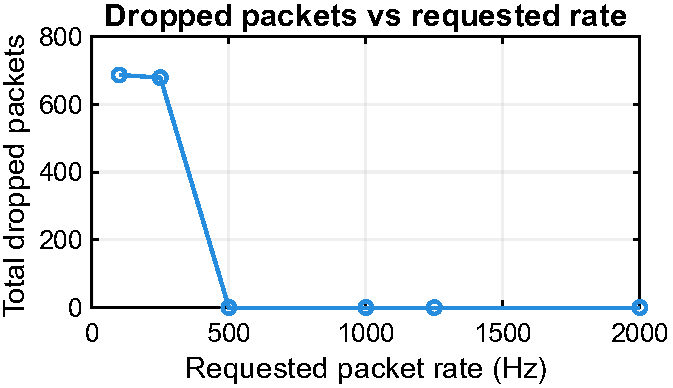
\includegraphics[width=0.95\linewidth]{images/Dropped packets vs requested rate.pdf}
		\caption{Dropped packets}
	\end{subfigure}
	\hfill
	\begin{subfigure}{0.48\textwidth}
		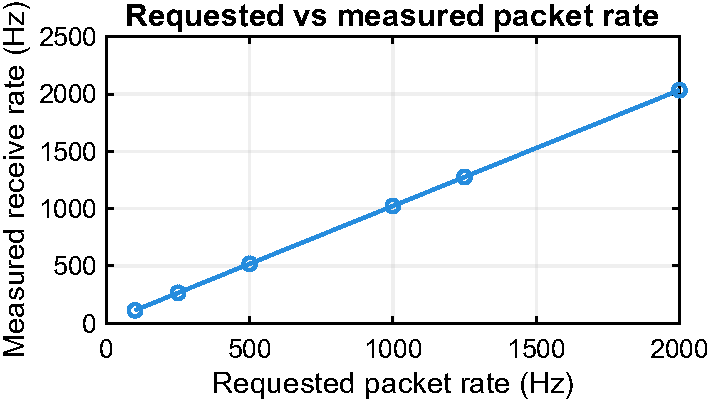
\includegraphics[width=0.95\linewidth]{images/Requested vs measured packet rate.pdf}
		\caption{Rate tracking}
	\end{subfigure}
	
	\caption{
		Communication performance across transmission rates. Packet loss occurred only at low frequencies, while measured receive rate tracked the requested rate approximately linearly.
	}
	\label{fig:comm_overview}
\end{figure}

Inter-arrival jitter, measured as the standard deviation of packet inter-arrival time, was present in all tests, with standard deviation decreasing as the requested rate increased, as shown in Fig.~\ref{fig:jitter}. However, percentile analysis revealed that occasional large timing excursions persisted even at higher rates, indicating intermittent latency spikes. While average jitter decreased with increasing rate, worst-case timing excursions remained present.

\begin{figure}[htbp]
	\centering
	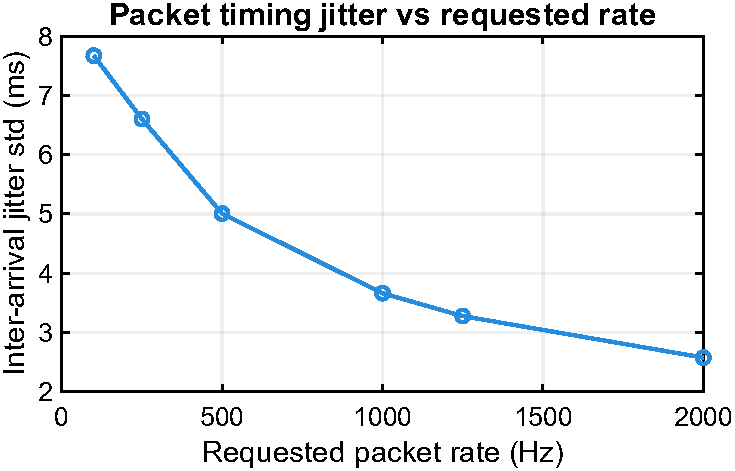
\includegraphics[width=0.58\textwidth]{images/Packet timing jitter vs requested rate.pdf}
	\caption{
		Packet inter-arrival jitter decreases with requested rate, although occasional large timing excursions remain present.
	}
	\label{fig:jitter}
\end{figure}

Overall, the serial link supported nominal packet throughput at or above 1~kHz with negligible packet loss in the tested configuration. This result describes packet generation and throughput, rather than low-latency delivery or 1\,ms closed-loop state freshness.

\subsubsection{Round-Trip Latency Results} \label{sec:results_rtt}
Round-trip latency results were highly consistent across all tested ping intervals. For nominal transmission intervals of 1~ms, 2~ms, and 10~ms, the success rate was 100\% in all cases, with no timeouts observed over 1000 samples per test.
The mean measured round-trip latency remained approximately constant across all three test conditions, with values of 15.60~ms, 15.64~ms, and 15.67~ms respectively. Similarly, the 95th and 99th percentile RTT values were tightly grouped around 16.2--16.4~ms, indicating consistent and predictable timing behaviour across repeated measurements. This behaviour is further illustrated in Fig.~\ref{fig:rtt_cdf}, where the cumulative distributions for all three tests overlap closely and rise sharply at approximately 15--16~ms, indicating that RTT is largely independent of the selected ping interval.

\begin{figure}[htbp]
	\centering
	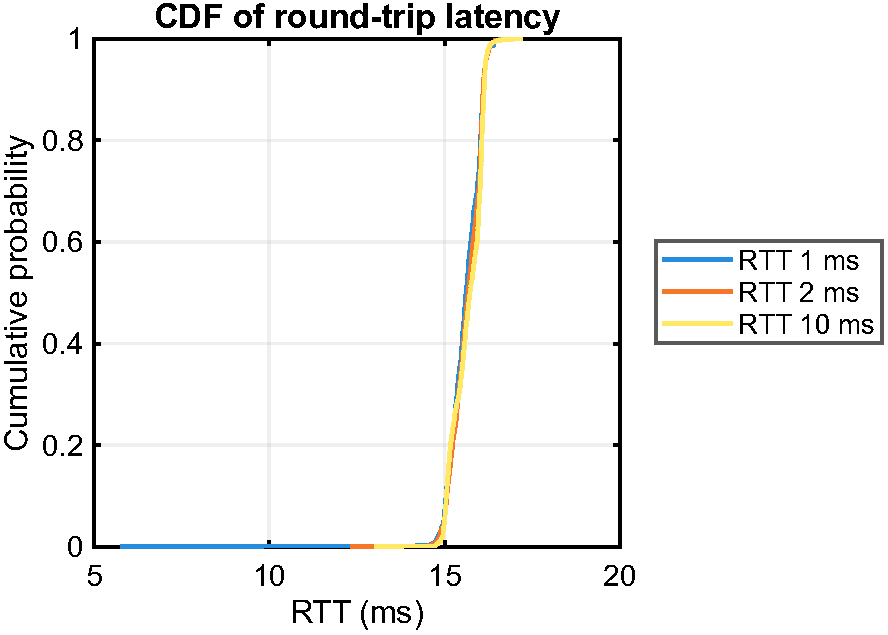
\includegraphics[width=0.6\textwidth]{images/CDF of round-trip latency.pdf}
	\caption{
		Cumulative distributions of RTT for 1~ms, 2~ms, and 10~ms ping intervals. The overlapping curves indicate a largely fixed 15--16~ms delay component.
	}
	\label{fig:rtt_cdf}
\end{figure}

The standard deviation of RTT remained below 0.52~ms in all cases, suggesting relatively low variability in round-trip timing. Minimum and maximum observed RTT values showed occasional larger deviations from the typical latency range, particularly in the 1~ms test, but these did not significantly affect the overall distribution.

These results indicate that RTT was dominated by a largely fixed delay component and changed little with ping interval. The measured delay remained predictable due to low variability and zero observed timeouts.

\subsubsection{End-to-End Host-Side Timing Results} \label{sec:results_host_timing}
End-to-end timing behaviour of the integrated haptic pipeline was evaluated using runtime logging of matched state-command cycles and raw parsed state packets.

Analysis of \texttt{device\_timing.csv} showed that all recorded control cycles were successfully matched, with a matched fraction of 1.000, indicating consistent correspondence between received state packets and transmitted torque commands.

The host-side end-to-end latency, defined as the time between state-packet parsing and completion of torque command transmission, was found to be low. The mean latency was 0.299~ms, with a median of 0.104~ms. The 95th percentile latency was 0.546~ms, and the 99th percentile was 2.04~ms, with a maximum observed latency of 3.35~ms. As shown in Fig.~\ref{fig:e2e_hist}, the distribution was concentrated at low values, with prominent peaks near 0~ms and around 0.5~ms, and only a limited number of higher-latency events.

\begin{figure}[htbp]
	\centering
	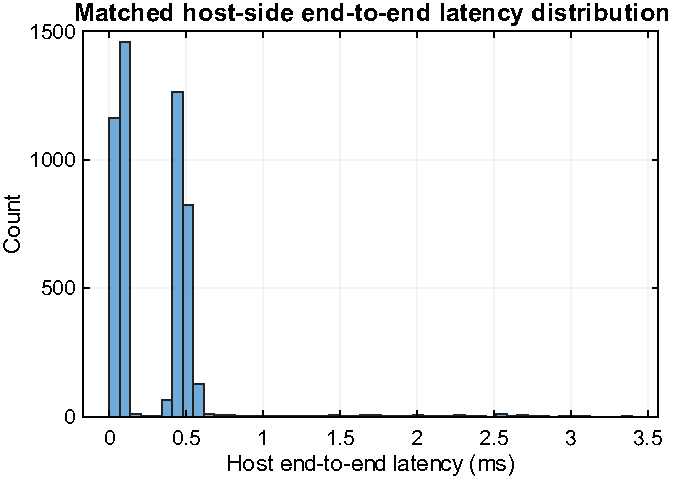
\includegraphics[width=0.64\textwidth]{images/Matched host-side end-to-end latency distribution.pdf}
	\caption{
		Matched host-side latency from state-packet parsing to torque-command transmission, concentrated at low values with few higher-latency outliers.
	}
	\label{fig:e2e_hist}
\end{figure}

Breakdown of intermediate pipeline delays showed that the majority of this latency was associated with serial transmission. The mean transmission duration was 0.249~ms, while the delay associated with publishing tool state and processing the haptic pipeline remained small, with mean values of 0.024~ms and 0.0044~ms respectively. This indicates that host-side computation and message-passing overhead were negligible relative to communication time.

Sequence analysis showed that command sequence progression remained consistent, with a mean command sequence gap of 1.14 and a maximum of 6, indicating that command updates were generally applied sequentially with minimal skipping. In contrast, the matched state sequence gap was significantly larger, with a mean of 33.45. This reflects the fact that the control loop operated on a subset of the available incoming state packets rather than processing every parsed packet. Here, sequence gap denotes the difference between consecutive sequence identifiers, such that a value of 1 corresponds to consecutive packets or commands and larger values indicate skipped intermediate sequence numbers.

A total of 54\,161 valid state packets were parsed during the test, compared to 5\,048 matched control cycles, confirming that the control loop operated on a subset of the incoming packet stream rather than consuming every parsed packet. The estimated parsed packet rate, computed from the mean host-side inter-arrival time, was approximately 1006~Hz, which is close to the expected 1~kHz transmission rate.

Analysis of host-side parsed-packet inter-arrival timing revealed significant variability. The mean inter-arrival time was 0.994~ms, but the median was only 0.0016~ms, reflecting that many packets were processed in immediate succession within bursts. The large difference between mean and median inter-arrival time indicates that packets were frequently processed in rapid bursts following periods of delay, rather than arriving at uniform intervals. This behaviour is illustrated in Fig.~\ref{fig:raw_host_hist}, where a dominant peak near 0~ms is accompanied by a much smaller secondary concentration around 14--16~ms. The 95th and 99th percentile inter-arrival times were 14.5~ms and 15.8~ms respectively, confirming the presence of intermittent host-side stalls.

\begin{figure}[htbp]
	\centering
	\includegraphics[width=1.0\textwidth]{images/Raw parsed state packet inter-arrival distribution(final).pdf}
	\caption{
		Host-side parsed-packet inter-arrival distribution. The secondary peak corresponds to the 95th--99th percentile range of 14.5--15.8~ms.
	}
	\label{fig:raw_host_hist}
\end{figure}

Despite this non-uniform host-side processing pattern, analysis of MCU-side timestamps showed that the embedded system generated state packets at a consistent rate. The effective MCU period per state was approximately 1.00~ms, corresponding to a nominal packet generation rate of 1000~Hz, with very low variability.

Taken together, the embedded controller generated packets at a regular rate, while host-side packet timing was non-uniform. Host-side processing latency nevertheless remained low. These results separate local packet generation and host computation from the effective age of the state used for haptic feedback.

\subsection{Simulation Validation Results}

Simulation validation was performed as described in Section~\ref{sec:method_simulation}, with actuator output disabled. These tests evaluated the haptic rendering model independently of physical actuator dynamics.

\subsubsection{Virtual Wall Contact Response} \label{sec:results_virtual_wall}

The virtual wall response was evaluated using a single-depth hold test. During contact, the rendered force magnitude had a mean value of 11.46~N and a standard deviation of 0.30~N, corresponding to a coefficient of variation of 0.026.

As shown in Fig.~\ref{fig:single_depth_contact}, force was generated only when the end-effector penetrated the virtual wall. When the end-effector was outside the wall, the output force remained approximately zero.

\begin{figure}[htbp]
	\centering
	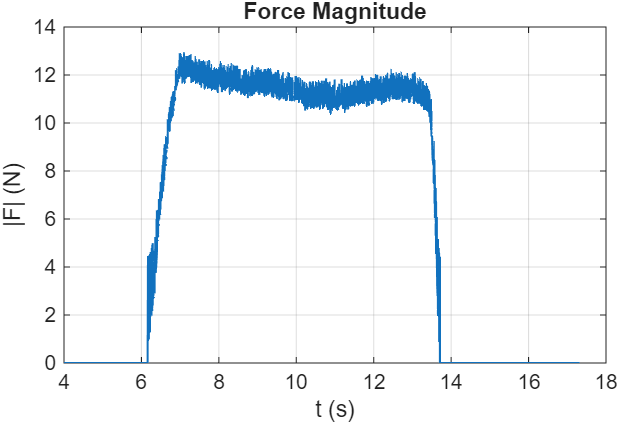
\includegraphics[width=0.58\textwidth]{images/SingleDepth_Force_Vs_Time.png}
	\caption{
		Single-depth virtual wall contact test. The rendered \( |\mathbf{F}| \) remains steady during sustained contact, with mean 11.46~N, standard deviation 0.30~N, and coefficient of variation 0.026.
	}
	\label{fig:single_depth_contact}
\end{figure}

\subsubsection{Force--Penetration Characterisation} \label{sec:results_force_penetration}

A multi-depth hold test was used to quantify the relationship between virtual penetration depth and logged rendered-force magnitude. A linear fit to the force--penetration data produced an effective stiffness of 489.57~N\,m$^{-1}$ with $R^2 = 0.9973$, as shown in Fig.~\ref{fig:force_penetration_fit}.

This closely matches the configured virtual coupling stiffness of 500~N\,m$^{-1}$ over the tested range.

\begin{figure}[htbp]
	\centering
	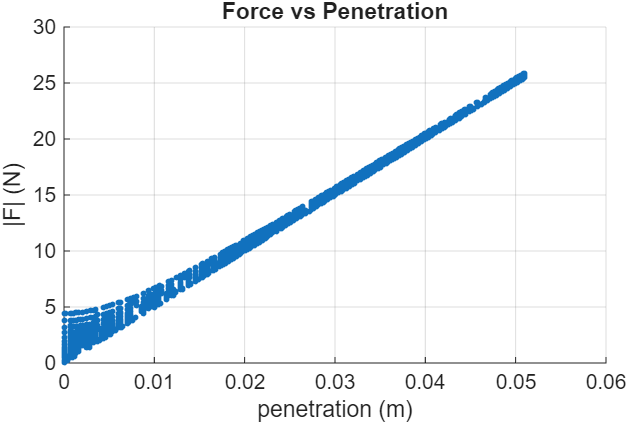
\includegraphics[width=0.58\textwidth]{images/MultiDepth_Force_Vs_Pen.png}
	\caption{
		Force--penetration relationship from the multi-depth hold test, with fitted stiffness 489.57~N\,m$^{-1}$ and $R^2 = 0.9973$.
	}
	\label{fig:force_penetration_fit}
\end{figure}

\subsubsection{Free-Space and Saturation Behaviour}

A no-contact test verified that the haptic engine produced no significant force output in free space.

A deep-penetration test was also performed to verify host-side force limiting. Under large penetration, the commanded force saturated at approximately 31~N, as shown in Fig.~\ref{fig:force_saturation}.

\begin{figure}[htbp]
	\centering
	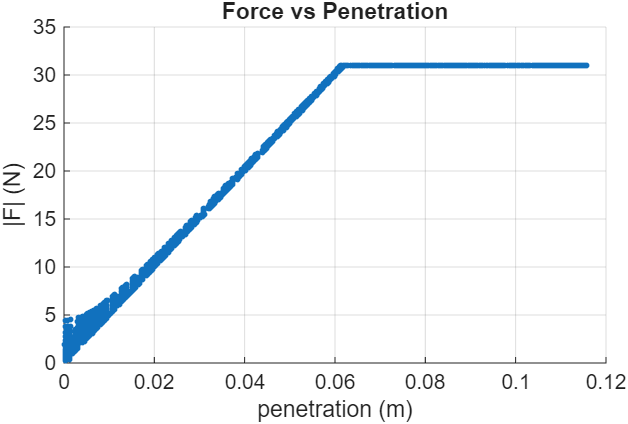
\includegraphics[width=0.58\textwidth]{images/Saturated_Force_Vs_Pen.png}
	\caption{
		Deep-penetration simulation test showing force saturation at the host-side limit of approximately 31~N.
	}
	\label{fig:force_saturation}
\end{figure}


\subsection{Safety Validation Results}

Safety validation evaluated whether torque commands remained bounded during high-force contact, rapid command transitions, and communication loss.

\subsubsection{Torque Saturation}

Torque saturation was evaluated using the deep-penetration test. Host-side saturation occurred in 31.10\% of samples, with the maximum raw torque command reaching 9.35~N\,m before being clamped to 7.66~N\,m. On the device side, the maximum applied torque was limited to 6.50~N\,m, matching the configured firmware torque cap.

\begin{figure}[htbp]
	\centering
	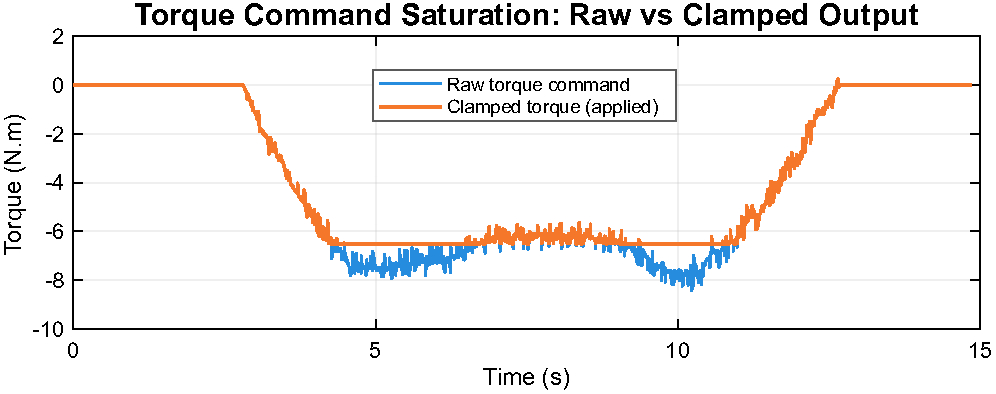
\includegraphics[width=0.65\textwidth]{images/Command and Applied Torque.pdf}
	\caption{
		Torque saturation during deep-penetration testing: raw host commands are clamped before transmission and applied torque remains bounded by the 6.50~N\,m firmware cap.
	}
	\label{fig:torque_saturation}
\end{figure}

\subsubsection{Rate Limiting} \label{sec:results_rate_limiting}

The embedded torque slew-rate limiter was evaluated from the applied torque logs. The measured 95th percentile slew rate was 55.000~N\,m\,s$^{-1}$, the 99th percentile was 55.005~N\,m\,s$^{-1}$, and the maximum measured slew rate was 55.010~N\,m\,s$^{-1}$. These values closely match the configured firmware limit of 55~N\,m\,s$^{-1}$.

The slew-rate distribution is shown in Fig.~\ref{fig:slew_hist}. The dominant peak at 0~N\,m\,s$^{-1}$ corresponds to steady-state operation, while the sharp upper bound occurs at the configured 55~N\,m\,s$^{-1}$ limit.

\begin{figure}[htbp]
	\centering
	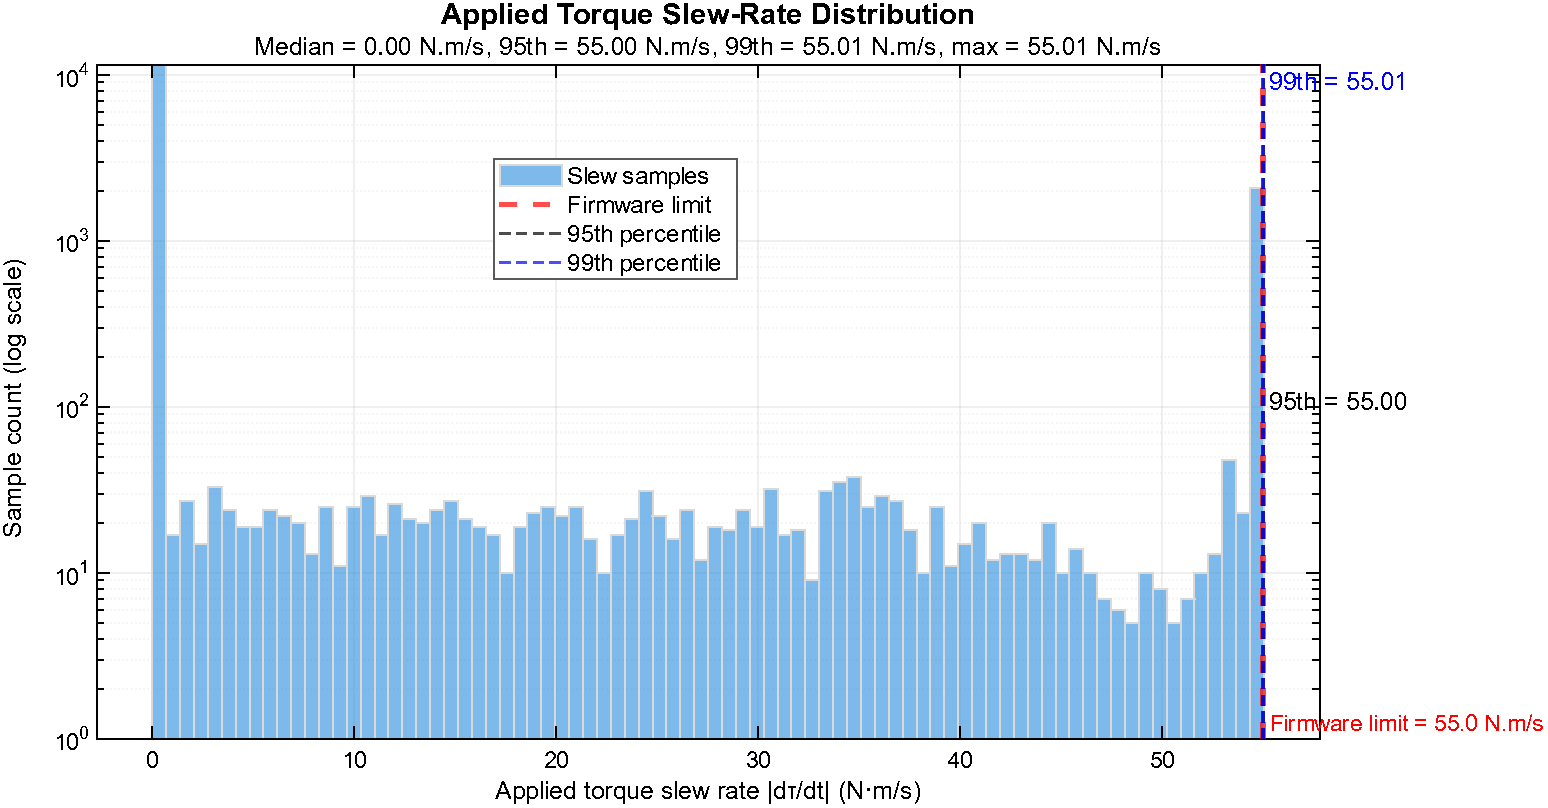
\includegraphics[width=0.74\textwidth]{images/Torque Slew Rate Distribution.pdf}
	\caption{
		Applied torque slew-rate histogram showing a sharp upper bound at the firmware limit of 55~N\,m\,s$^{-1}$.
	}
	\label{fig:slew_hist}
\end{figure}

\subsubsection{Watchdog Timeout Behaviour}

The watchdog was evaluated by deliberately interrupting host torque-command transmission. A total of 259 watchdog activation events were recorded, corresponding to 6.81\% of device samples. The total watchdog-active time was 0.529~s, with a mean activation duration of 0.0020~s and a maximum duration of 0.311~s.

As shown in Fig.~\ref{fig:watchdog}, applied torque was removed during watchdog activation.

\begin{figure}[htbp]
	\centering
	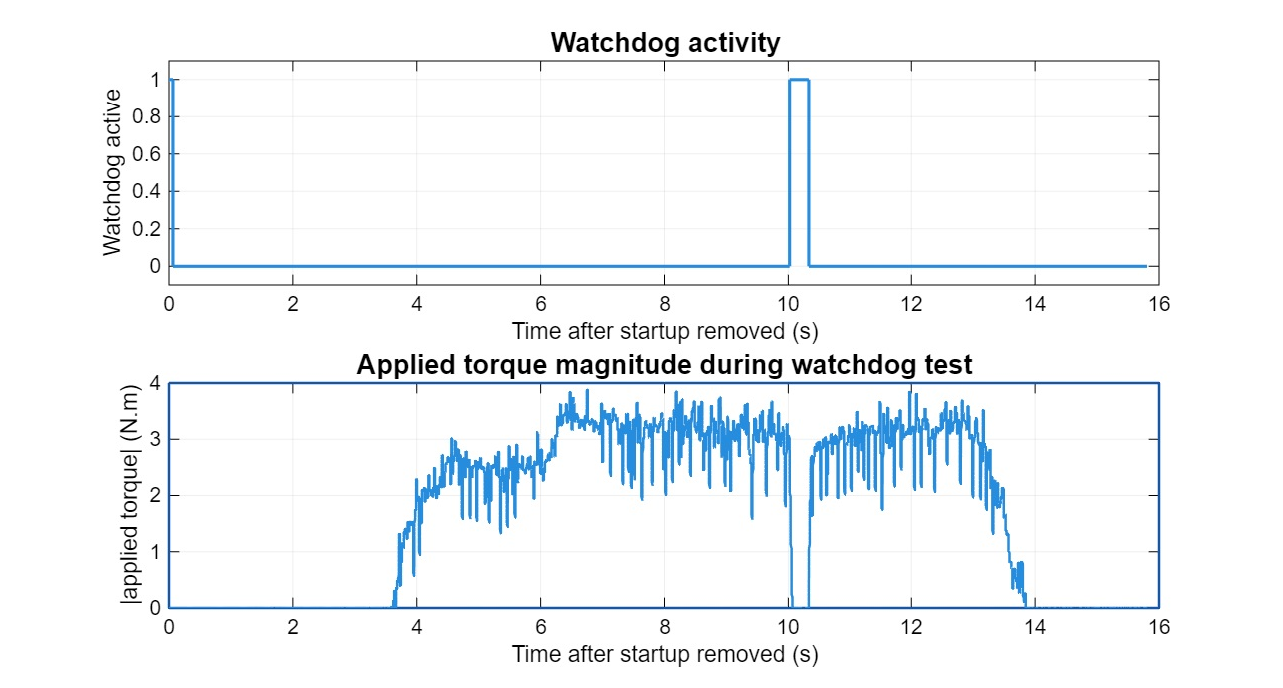
\includegraphics[width=0.74\textwidth]{images/Device Safety Validation - Watchdog Focus.pdf}
	\caption{
		Watchdog validation during interrupted host command transmission. Applied torque is removed when the watchdog becomes active.
	}
	\label{fig:watchdog}
\end{figure}

\subsubsection{Command Consistency}

Sequence-matched host and device logs showed a mean applied torque magnitude error of 0.134~N\,m between host commands and device-side applied torque. For typical commanded torques of approximately 2--4~N\,m, this corresponds to roughly 3--7\% error. Larger differences occurred during transient command changes, especially when the slew-rate limiter and safety clamps were active.


\subsection{Hardware Validation Results}

Hardware validation was performed with actuator feedback enabled. Because direct force sensing and current measurement were not available, these results quantify interaction behaviour using logged position, force-command, and torque-command data rather than calibrated physical force output. Final force-feedback testing was limited to single-axis actuation due to actuator failure, although both joints remained available for position sensing.

\subsubsection{Repeated Contact With Virtual Wall} \label{sec:results_stable_contact_hardware}

During repeated motor-enabled contact with the virtual wall, penetration remained bounded. The mean penetration depth was 0.0342~m, the 95th percentile penetration depth was 0.0498~m, and the maximum penetration depth was 0.0517~m.

The force--penetration relationship during this test remained approximately linear, with an effective stiffness of 490.99~N\,m$^{-1}$ and $R^2 = 0.9979$. This indicates that the rendered force command remained consistent with the virtual coupling model during closed-loop interaction.
The fitted stiffness of 490.99~N\,m$^{-1}$ agrees closely with the simulation-only result of 489.57~N\,m$^{-1}$ in Section~\ref{sec:results_force_penetration}. This comparison is based on logged command data rather than direct force measurement.

\begin{figure}[htbp]
	\centering
	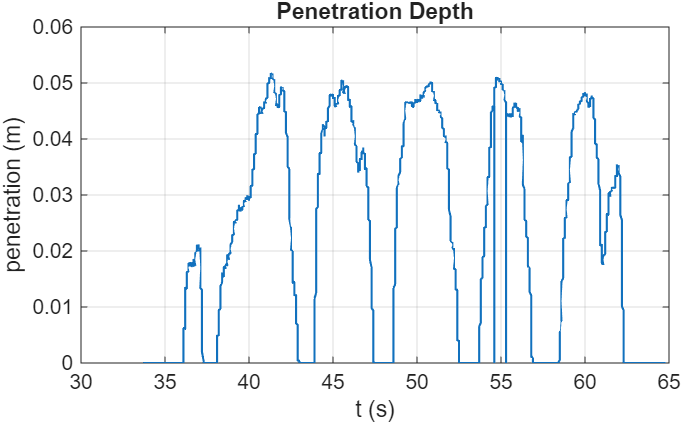
\includegraphics[width=0.58\textwidth]{images/MotorON_Pen_vs_Tine.png}
	\caption{
		Motor-enabled repeated contact test. Maximum penetration was approximately 0.052~m; the force--penetration fit gave 490.99~N\,m$^{-1}$ with $R^2=0.9979$.
	}
	\label{fig:motor_contact_penetration}
\end{figure}

\subsubsection{Constrained Motion Along a Surface}

Constrained motion was evaluated by bringing the end-effector into contact with the virtual wall and moving along the surface. Metrics were computed over the sustained-contact window from 20.50~s to 23.20~s, excluding entry and release transients. During this window, the mean penetration depth, computed from device--proxy separation, was 0.0492~m and the maximum penetration depth was 0.0512~m.

Force decomposition showed that the rendered force was predominantly normal to the surface, with a median $|F_n|/|F_t|$ ratio of 17.72 and a 95th percentile ratio of 266.03. The sustained-contact force magnitude had a mean value of 24.68~N and a standard deviation of 0.72~N, corresponding to a coefficient of variation of 0.029.

The device and proxy trajectories are shown in Fig.~\ref{fig:constrained_motion_traj}. The proxy remains aligned with the virtual wall, while the device trajectory shows bounded displacement normal to the wall and motion along the tangential direction.

\begin{figure}[H]
	\centering
	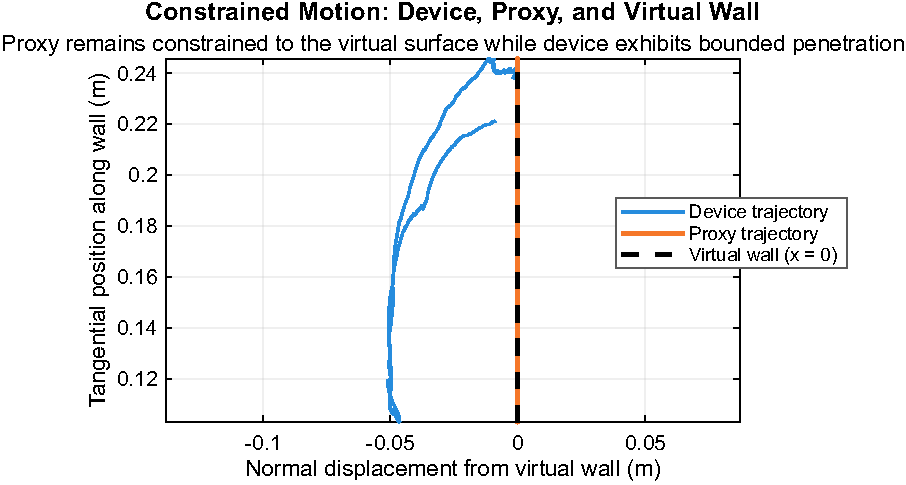
\includegraphics[width=0.7\textwidth]{images/Constrained Motion - Device, Proxy, and Virtual Wall.pdf}
	\caption{
		Device and proxy trajectories during the analysed constrained-motion window from 20.50~s to 23.20~s. The proxy remains constrained to the wall while device normal displacement stays bounded.
	}
	\label{fig:constrained_motion_traj}
\end{figure}

Across the motor-enabled hardware tests, penetration remained bounded and logged force-command behaviour remained approximately consistent with the implemented virtual coupling model.


%%%%%%%%%%%%%%%%%% DISCUSSION %%%%%%%%%%%%%%%%%%
\section{Discussion} \label{sec:discussion}
%Discussion section 
This section interprets the experimental results in terms of the main constraints on haptic performance: communication latency, delayed contact behaviour, hardware limitations, and the resulting design trade-offs.

\subsection{Communication and Latency Constraints} \label{sec:discussion_communication_latency}

The central finding from the communication evaluation is that transport delay, measured at 15.60--15.67\,ms mean round-trip with 95th and 99th percentiles around 16.2--16.4\,ms, is the dominant limitation on closed-loop performance. In contrast, host-side processing latency remained low (mean 0.299\,ms, 99th percentile 2.04\,ms), confirming that computation is not the bottleneck for the nominal 1\,kHz local haptic/device loops.

This delay directly bounds achievable haptic stiffness. As delay increases, phase lag reduces the stability margin and can inject artificial energy into the sampled-data loop \cite{colgatePassivityClassSampleddata1997}, so lower stiffness and additional damping are required. Consequently, the realised system renders compliant rather than rigid contact.

The ST-Link virtual COM interface was convenient for development, but the observed burst-like delivery pattern and low-rate packet loss suggest USB CDC buffering and host scheduling overhead that is large relative to the control timestep. Although the present work does not isolate every stage in the communication path, the evidence shows that communication architecture must be treated as a first-order design constraint alongside control and mechanical design.

The system should therefore be interpreted as a high-rate local haptic renderer operating over delayed sampled state, rather than as a true 1\,kHz end-to-end haptic loop. Snapshot channels reduce backlog-induced latency by ensuring that the haptic and device loops consume the newest available state, but they cannot remove transport delay, increase the physics-simulation update rate, or guarantee that the rendered contact state is physically fresh at 1\,ms intervals.

\subsection{Local Contact State Limitation} \label{sec:discussion_local_contact_state}

A further limitation of the realised architecture is that the nominal 1\,kHz haptic loop did not evolve a complete local contact state independently of the slower simulation and communication layers. It consumed latest-available snapshots of tool and world state, then recomputed proxy/contact information at each cycle. The renderer could therefore execute at high frequency, but the physical meaning of each update was still bounded by snapshot freshness and communication delay. The limitation was not the execution rate of the haptic computation, but that the rendered state was not itself evolved and validated at 1\,kHz across the full interaction loop.

A more complete architecture would maintain persistent proxy and local contact state inside the high-rate loop. Rather than re-projecting the proxy from scratch, the proxy would evolve continuously subject to contact constraints, preserving contact history, tangential motion, and release behaviour. This is closer to constraint-based proxy or god-object approaches \cite{zillesConstraintbasedGodobjectMethod1995,ruspiniHapticDisplayComplex1997,salisburyHapticRenderingSurfaces1997}. The simpler projection-based approach used here was sufficient to demonstrate bounded contact, but it limited contact smoothness and weakens any claim to true 1\,kHz end-to-end haptic interaction.

This clarifies the relationship between the haptic renderer and the physics engine. The physics engine provided the authoritative global scene state at a lower rate, while the haptic loop consumed snapshots of that state. A stronger version of this multi-rate design would allow the haptic loop to maintain a reduced local model of contacted objects at high frequency, while slower application, rendering, or physics subsystems provide broader scene updates and maintain global consistency, following the motivation of multilevel haptic rendering for complex environments \cite{ruspiniHapticDisplayComplex1997}.

\subsection{Observed Contact Behaviour Under Delay} \label{sec:discussion_stability}

Although communication timing was imperfect, the tested interactions remained bounded and controllable because snapshot channels used the newest available state rather than queued historical samples, thread separation avoided cross-subsystem blocking, and damping countered delayed feedback effects. Embedded torque rate limiting further prevented abrupt torque transitions that can excite oscillations. Watchdog activation data also show that communication interruptions were handled safely: 259 activation events were recorded, with a mean duration of 2\,ms and torque removed during activation (Section~\ref{sec:results}).

These mechanisms address the passivity concerns identified by Colgate and Schenkel \cite{colgatePassivityClassSampleddata1997} in a practical rather than formal way. The results provide evidence of bounded behaviour in the tested cases, not a passivity proof. Contact therefore remained controllable without divergent motion or sustained oscillation, but the compliant feel was still a direct consequence of delayed feedback; rigid contact cannot be achieved under the measured latency conditions by force-model tuning alone.

\subsection{Hardware Limitations} \label{sec:discussion_hardware_limitations}
The hardware results must be interpreted within clear prototype constraints. The most important was the absence of current sensing. The initial design targeted STM32 B-G431-ESC1 motor drivers, but integration with the selected magnetic encoders proved unreliable within the project timescale. SimpleFOC Mini modules provided a more robust integration path, but left torque control effectively open-loop with respect to current. As a result, commanded torque cannot be interpreted as calibrated physical torque, and the hardware evaluation should be read primarily as evidence of logged command consistency and qualitative interaction capability. This limitation does not affect the communication, timing, and bounded-contact results, which do not depend on absolute force calibration.

A second limitation was the GT2 belt reduction used to increase base-joint torque. The belt improved available torque but slipped under high load, even after adding an adjustable idler pulley, probably because 3D-printed pulleys did not provide manufactured tooth-profile precision. Actuator torque limits would still bound force output even without slip, directly constraining renderable stiffness.

A further limitation arose from the failure of one actuator during development. Final hardware validation therefore used single-joint actuation with two-joint sensing, so conclusions about full 2-DOF force rendering remain provisional. Overall, actuator capability and transmission design impose significant constraints alongside communication latency in low-cost haptic systems.

\subsection{Design Trade-Offs} \label{sec:discussion_design_tradeoffs}
The system therefore reflects a trade-off between bounded contact behaviour, responsiveness, and force fidelity. Damping and torque rate limiting avoided abrupt or divergent responses, but reduced perceived stiffness. The measured limiter of approximately 55~N\,m\,s$^{-1}$ implies an approximate 0.13~s rise time to reach the 7~N\,m torque range, so hard contacts feel gradual rather than instantaneous.

An additional perceptual limitation was observed at contact release: after sustained penetration into a virtual wall, the transition back to free motion could feel slightly jerky. This may be associated with abrupt proxy-state changes, lag in the filtered proxy velocity state, or delayed torque commands. The implemented approach therefore prioritised controllability over maximum stiffness, showing that high-fidelity force rendering cannot be improved by optimising one subsystem in isolation.

\subsection{Project Management and Development Process} \label{sec:discussion_project_management}

The project plan provided a useful structure, but the final Gantt chart in Appendix~\ref{app:gantt} reflects an adaptive process shaped by integration risk. The main management decision was to prioritise a working system-level prototype over ideal subsystem performance: driver integration difficulties led to SimpleFOC Mini modules, and later actuator failure shifted final validation from full 2-DOF force feedback to single-axis actuation with two-axis sensing. Risk management therefore focused on preserving the communication, simulation, safety, and bounded-contact evaluation objectives through staged testing, torque limiting, slew-rate limiting, and watchdog safety.



%%%%%%%%%%%%%%%%%% CONCLUSION %%%%%%%%%%%%%%%%%%
\section{Conclusions and Future Work} \label{sec:conclusion}
\noindent
This section summarises the extent to which the project objectives were achieved and identifies the most important directions for future development.

\subsection{Conclusions}

This project presented the design, implementation, and evaluation of a low-cost, modular haptic rendering system integrating a two-degree-of-freedom input device with a custom real-time simulation and visualisation framework.
The system successfully achieved its primary objective of enabling bidirectional interaction between a user-operated device and a virtual environment, with real-time computation of interaction forces and feedback through actuator torque control. The architecture was designed to prioritise modularity and extensibility, allowing clear separation between hardware, communication, simulation, and rendering subsystems.

Experimental evaluation showed that selected local subsystems could operate at nominal 1\,kHz rates, including embedded packet generation and host-side haptic/device-loop execution, with low host-side processing latency. However, the complete bidirectional haptic interaction should not be claimed as a true 1\,kHz end-to-end loop, because force computation operated on latest-available snapshots affected by communication delay and asynchronous simulation timing. The dominant limitation was the 15.60--15.67\,ms round-trip communication delay, which bounded achievable virtual stiffness.
Within this constraint, bounded and controllable contact interaction was observed during the tested interactions through a combination of architectural and control strategies, including snapshot-based communication and damping-based stabilisation. The resulting haptic feedback was usable and controllable, but not rigid or quantitatively force-calibrated, due to finite actuator torque, the absence of current sensing, belt slip under high load, and the limitation to single-axis actuation during final validation.

The project outcomes address the objectives defined in Section~\ref{sec:introduction}. A sub-£200 haptic interface was constructed with joint sensing and motor command capability, although final actuation was limited to one joint after actuator failure. The system demonstrated nominal 1\,kHz packet streaming while separately quantifying packet loss, out-of-order events, burst-like delivery, RTT, and host-side processing latency. Logged simulated rendered-force data gave an effective stiffness of 489.57\,N\,m$^{-1}$, within 5\% of the configured 500\,N\,m$^{-1}$ value, with $R^2=0.9973$. Saturation, torque limiting, slew-rate limiting, watchdog behaviour, motor-enabled contact, and constrained-motion tests were also validated, while documenting the communication, actuation, sensing, and mechanical limitations that affect generalisation.

Overall, the project demonstrates that bounded and usable haptic interaction can be achieved using low-cost hardware and a modular software architecture, even in the presence of significant communication latency. The main insight is that high-rate local control and an accurate command-side force model are not sufficient on their own: communication delay, actuator capability, transmission design, and the absence of a persistent high-rate local contact-state model jointly determine achievable haptic fidelity.

\subsection{Future Work}
A key priority is reducing communication latency. The current ST-Link virtual COM pathway appears to introduce buffering and scheduling delays that dominate the closed-loop response, so future work should compare lower-latency alternatives such as direct UART via a dedicated USB--UART bridge, native USB bulk transfer, CAN bus, or Ethernet-based communication.

Future work should extend the existing multi-rate architecture so that the haptic loop maintains a reduced local model of currently contacted objects at 1\,kHz, while slower physics, rendering, or application layers remain responsible for broader scene evolution and consistency. The high-rate loop would continuously evolve the proxy, contact manifold, and local object interaction state, reducing dependence on low-rate world snapshots and improving contact continuity, following the motivation of multilevel haptic rendering for complex environments \cite{ruspiniHapticDisplayComplex1997}.

A related extension would be to move the haptic rendering loop, or at least the local contact/proxy evolution, onto the embedded controller. Communication with the host would then focus on object interaction parameters, local contact primitives, or periodic scene-state updates, rather than every force update depending on a delayed host--device exchange. This would lower effective actuator-side latency, with the trade-off that the embedded model would need to be simplified using local planes, SDF patches, virtual fixtures, or reduced contact geometry.

On the control side, incorporating task-space dynamics using an operational-space formulation \cite{khatibUnifiedApproachMotion1987a} would allow the manipulator's inertia and dynamics to be compensated during interaction, improving force-rendering transparency.

Hardware improvements are also important. Current sensing, together with external force measurement, would enable more accurate torque control, quantitative physical force validation, and more advanced impedance or operational-space control. Transmission design could be improved by replacing the slipping GT2 belt stage with a lower-backlash alternative such as a capstan drive, while higher-torque actuators and restored two-degree-of-freedom actuation would improve interaction realism.

Further improvements to the haptic rendering model could address the force-direction inconsistencies observed during large penetration. Constraint-based contact solvers could enforce continuous proxy motion across timesteps, reducing surface-normal discontinuities caused by re-projecting the proxy from scratch. Contact entry and exit transitions should also be smoothed by blending proxy velocity state across release and discarding stale torque commands before they affect the user.

From a software and evaluation perspective, integration with platforms such as NVIDIA Isaac Sim or MATLAB/Simulink would enable more realistic robotic scenarios, while quantitative force measurement, user studies, and task-based metrics would better assess effectiveness as a training tool.

Together, these developments would enable the system to evolve from a low-cost prototype into a more capable and general-purpose haptic interface platform for robotic interaction and training applications.


\label{endofmain}
Page \thepage\ of \pageref{endofmain}
%%%%%%%%%%%%%%%%%% REFERENCES %%%%%%%%%%%%%%%%%%
\clearpage % uncomment to start on a new page if wanted
\printbibliography[title={References},heading=bibintoc] % a single list of references for the whole thesis



%%%%%%%%%%%%%%%%%% APPENDICES %%%%%%%%%%%%%%%%%%
\begin{uomappendix}
	\section{Preliminary Project Proposal}
	\begin{figure}[H]
		\centering
		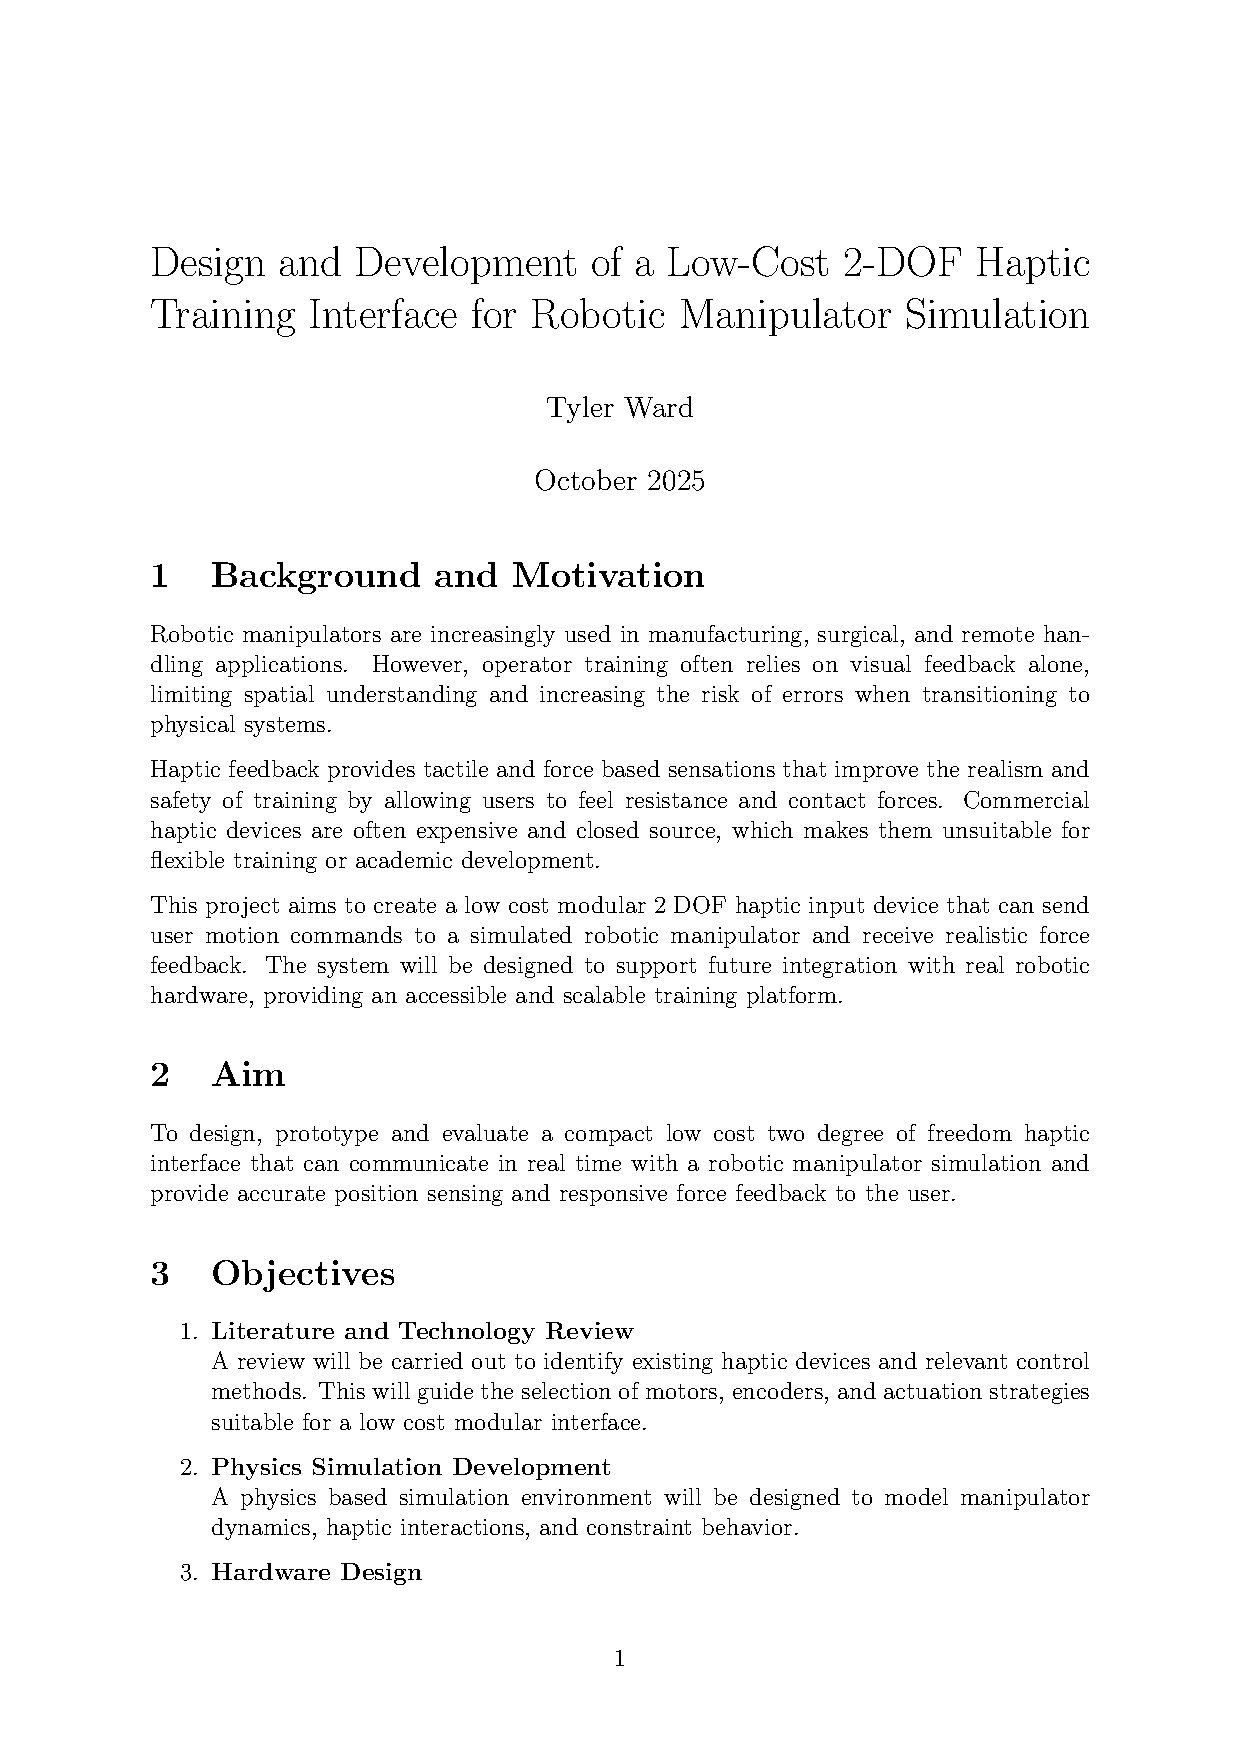
\includegraphics[width=0.7\linewidth]{images/Preliminary_Project_Proposal}
		\caption{Original project outline as submitted at the start of the project}
		\label{fig:preliminaryprojectproposal}
	\end{figure}

	


\begin{landscape}
	
\section{Gantt Chart} \label{app:gantt}
\begin{figure}[H]
	\centering
	\includegraphics[angle=0,height=0.80\textheight]{"images/gantt"}
	\caption{Final Gantt chart showing the execution of the project over time. The chart reflects the iterative development process, including overlapping software and hardware work, as well as deviations from the original plan due to motor driver integration issues, hardware delays, and subsystem integration challenges.}
	\label{fig:gantt}
\end{figure}


\section{Risk Register and Health \& Safety Risk Assessment} \label{app:risk_assesment}
\begin{figure}[H]
	\centering
	\includegraphics[angle=0,height=0.80\textheight]{"images/Risk Register Template"}
	\caption{Project Risk Assessment}
	\label{fig:risk-register}
\end{figure}

\section{CPD Log} \label{app:cpd_log}
\begin{figure}[H]
	\centering
	\includegraphics[angle=0,height=0.80\textheight]{"images/cpd"}
	\caption{CPD Log documenting skills and knowledge acquired during the project.}
	\label{fig:cpd}
\end{figure}

\end{landscape}
%	\begin{figure}[t]
%		\centering
%		\resizebox{\textwidth}{!}{%
%			\begin{tikzpicture}[
%				font=\small,
%				thread/.style={draw, rounded corners, very thick, minimum width=3.3cm, minimum height=10.8cm, fill=gray!6},
%				block/.style={draw, rounded corners, align=center, minimum width=2.7cm, minimum height=1.35cm, fill=white},
%				extblock/.style={draw, rounded corners, align=center, minimum width=2.8cm, minimum height=1.35cm, fill=blue!4},
%				data/.style={draw, rounded corners, align=center, minimum width=2.2cm, minimum height=0.85cm, fill=green!6},
%				arrowq/.style={->, thick},
%				snaparrow/.style={->, thick, dashed},
%				note/.style={align=center, font=\scriptsize}
%				]
%				
%				% Swimlanes
%				\node[thread] (renderlane) at (0,0) {};
%				\node[thread] (simlane)    at (4.2,0) {};
%				\node[thread] (haptlane)   at (8.4,0) {};
%				\node[thread] (devlane)    at (12.6,0) {};
%				\node[thread] (loglane)    at (16.8,0) {};
%				
%				% Lane titles
%				\node[font=\bfseries] at (renderlane.north) [yshift=-0.45cm] {Render Thread};
%				\node[font=\bfseries] at (simlane.north)    [yshift=-0.45cm] {Simulation Thread};
%				\node[font=\bfseries] at (haptlane.north)   [yshift=-0.45cm] {Haptics Thread};
%				\node[font=\bfseries] at (devlane.north)    [yshift=-0.45cm] {Device Thread};
%				\node[font=\bfseries] at (loglane.north)    [yshift=-0.45cm] {Logging Thread};
%				
%				% Thread rate labels
%				\node[note] at (8.4,4.2) {1 kHz};
%				\node[note] at (12.6,4.2) {1 kHz};
%				\node[note] at (4.2,4.2) {fixed $dt = 1/240$ s};
%				
%				% Render lane blocks
%				\node[block] (window) at (0,2.2) {\textbf{Window / UI}\\\scriptsize OpenGL window\\\scriptsize ImGui controls};
%				\node[block] (renderer) at (0,0.2) {\textbf{GlSceneRenderer}\\\scriptsize scene rendering\\\scriptsize tool/proxy visualisation};
%				
%				% Simulation lane blocks
%				\node[block] (world) at (4.2,1.4) {\textbf{WorldManager}\\\scriptsize authoritative scene state\\\scriptsize applies commands / builds snapshots};
%				\node[block] (physx) at (4.2,-1.2) {\textbf{PhysicsEnginePhysX}\\\scriptsize fixed-step rigid-body simulation\\\scriptsize applies haptic interaction forces};
%				
%				% Haptics lane blocks
%				\node[block] (haptic) at (8.4,0.1) {\textbf{HapticEngine}\\\scriptsize SDF contact query\\\scriptsize proxy projection\\\scriptsize virtual coupling + force clamp};
%				
%				% Device lane blocks
%				\node[block] (device) at (12.6,0.1) {\textbf{DeviceAdapter}\\\scriptsize serial RX/TX + packet parsing\\\scriptsize FK pose estimation\\\scriptsize Jacobian transpose torque mapping};
%				
%				% Logging lane blocks
%				\node[block] (logger) at (16.8,0.8) {\textbf{Logger Thread}\\\scriptsize drains log channels\\\scriptsize writes files on shutdown};
%				\node[data] (csv1) at (16.8,-1.2) {\texttt{device\_timing.csv}};
%				\node[data] (csv2) at (16.8,-2.5) {\texttt{device\_state\_log.csv}};
%				
%				% Physical system to right
%				\node[extblock] (user) at (21.0,2.2) {\textbf{User}};
%				\node[extblock] (pdev) at (21.0,0.4) {\textbf{2-DOF Haptic Device}\\\scriptsize encoders + BLDC actuators};
%				\node[extblock] (fw) at (21.0,-1.7) {\textbf{Embedded Firmware}\\\scriptsize device state packets\\\scriptsize torque execution / watchdog};
%				
%				% Internal simulation arrows
%				\draw[arrowq] (world) -- node[right, font=\scriptsize] {world state / rebuilds} (physx);
%				\draw[arrowq] (physx) -- node[left, font=\scriptsize] {updated poses} (world);
%				
%				% Commands from UI
%				\draw[arrowq] (renderer.east) to[out=10,in=170] node[above, font=\scriptsize] {WorldCommand} (world.west);
%				
%				% World snapshots
%				\draw[snaparrow] (world.east) to[out=10,in=170] node[above, font=\scriptsize] {WorldSnapshot} (haptic.west);
%				\draw[snaparrow] (world.west) to[out=170,in=10] node[above, font=\scriptsize] {WorldSnapshot} (renderer.east);
%				
%				% Haptic snapshot to renderer
%				\draw[arrowq] (haptic.west) to[out=160,in=-10] node[below, font=\scriptsize] {HapticSnapshotMsg} (renderer.east);
%				
%				% Wrench to physics
%				\draw[arrowq] (haptic.west) to[out=200,in=20] node[below, font=\scriptsize] {HapticWrenchCmd} (physx.east);
%				
%				% Device thread links
%				\draw[arrowq] (device.west) to[out=180,in=0] node[above, font=\scriptsize] {ToolStateMsg} (haptic.east);
%				\draw[arrowq] (haptic.east) to[out=0,in=180] node[below, font=\scriptsize] {HapticWrenchCmd} (device.west);
%				
%				% Logging links
%				\draw[arrowq] (device.east) to[out=0,in=180] node[above, font=\scriptsize] {DeviceTimingLogMsg} (logger.west);
%				\draw[arrowq] (device.east) to[out=-10,in=180] node[below, font=\scriptsize] {DeviceStateLogMsg} (logger.west);
%				\draw[arrowq] (logger) -- (csv1);
%				\draw[arrowq] (logger) -- (csv2);
%				
%				% Physical closed loop
%				\draw[arrowq] (device.east) to[out=0,in=180] node[above, font=\scriptsize] {TorqueCommandPacket} (fw.west);
%				\draw[arrowq] (fw.west) to[out=180,in=0] node[below, font=\scriptsize] {DeviceStatePacket} (device.east);
%				
%				\draw[arrowq] (user) -- node[right, font=\scriptsize] {motion / felt force} (pdev);
%				\draw[arrowq] (pdev) -- (fw);
%				
%				% Legend
%				\node[draw, rounded corners, align=left, fill=white] at (8.8,-5.2) {%
%					\scriptsize \textbf{Legend}\\
%					\scriptsize Solid arrows: queued messages / commands\\
%					\scriptsize Dashed arrows: latest-value snapshot channels
%				};
%				
%			\end{tikzpicture}%
%		}
%		\caption{Host-side software architecture and data flow. The system is partitioned into rendering, simulation, haptic, device communication, and logging threads. The haptic loop consumes the latest tool state and world snapshot, computes contact forces, and publishes interaction commands both to the physics engine and to the device adapter for torque rendering.}
%		\label{fig:sd}
%	\end{figure}

	%\subsection{Other appendices as necessary}
\begin{landscape}
	\section{Mechanical Design Drawing}
	\label{app:mechanical_design}
	
	\centering
	
	\rotatebox{0}{%
		\begin{minipage}{0.95\textheight}
			\centering
			\includegraphics[height=0.80\textheight]{"images/V2 Base Drawing v1"}
			
			\captionof{figure}{CAD assembly of the 2-DOF haptic interface illustrating link geometry, actuator configuration, belt-driven base joint, and encoder placement. Link dimensions are annotated to define the kinematic model used for forward kinematics and Jacobian-based torque mapping.}
			\label{fig:v2-base-drawing-v1}
		\end{minipage}
	}
	
\end{landscape}

\section{Source Code and Repository Information}
	Repository Link: \href{https://github.com/TylerWardUOM/3rd-yr-project}{3rd-yr-project} \\
	
	Below is the README for the repo:
	\begingroup
	\markdownSetup{
		renderers = {
			headingOne = {\section*{#1}},
			headingTwo = {\subsection*{#1}},
			headingThree = {\subsubsection*{#1}},
			headingFour = {\paragraph*{#1}}
		}
	}
	\markdownInput{README.md}
	\endgroup
\end{uomappendix}


%%%%%%%%%%%%%%%%%% END MATTER %%%%%%%%%%%%%%%%%%
\end{document}
